\documentclass[12pt,bibliography=oldstyle,DIV=12,parskip=half-]{scrreprt}
\newif\iflatexml\latexmlfalse
\usepackage{xstring}
\newcommand{\includePrueba}[1]{\input{#1}}
\newcommand{\includeFileOrFigure}[1]{%
  \IfBeginWith{#1}{figures/}{%
    \begin{figure}[H]
      \figureStyle
      \StrBefore[2]{#1}{/}[\temp]
      \tikzsetnextfilename{figures/femigracion/femigracion}
\begin{tikzpicture}[
    font=\footnotesize,
    thick
  ]
\usetikzlibrary{positioning,fit,calc,shapes}
\def\nw{1cm}

\makeatletter
\pgfkeys{/pgf/.cd,
  parallelepiped offset x/.initial=2mm,
  parallelepiped offset y/.initial=2mm
}
\pgfdeclareshape{parallelepiped}
{
  \inheritsavedanchors[from=rectangle] % this is nearly a rectangle
  \inheritanchorborder[from=rectangle]
  \inheritanchor[from=rectangle]{north}
  \inheritanchor[from=rectangle]{north west}
  \inheritanchor[from=rectangle]{north east}
  \inheritanchor[from=rectangle]{center}
  \inheritanchor[from=rectangle]{west}
  \inheritanchor[from=rectangle]{east}
  \inheritanchor[from=rectangle]{mid}
  \inheritanchor[from=rectangle]{mid west}
  \inheritanchor[from=rectangle]{mid east}
  \inheritanchor[from=rectangle]{base}
  \inheritanchor[from=rectangle]{base west}
  \inheritanchor[from=rectangle]{base east}
  \inheritanchor[from=rectangle]{south}
  \inheritanchor[from=rectangle]{south west}
  \inheritanchor[from=rectangle]{south east}
  \backgroundpath{
    % store lower right in xa/ya and upper right in xb/yb
    \southwest \pgf@xa=\pgf@x \pgf@ya=\pgf@y
    \northeast \pgf@xb=\pgf@x \pgf@yb=\pgf@y
    \pgfmathsetlength\pgfutil@tempdima{\pgfkeysvalueof{/pgf/parallelepiped offset x}}
    \pgfmathsetlength\pgfutil@tempdimb{\pgfkeysvalueof{/pgf/parallelepiped offset y}}
    \def\ppd@offset{\pgfpoint{\pgfutil@tempdima}{\pgfutil@tempdimb}}
    \pgfpathmoveto{\pgfqpoint{\pgf@xa}{\pgf@ya}}
    \pgfpathlineto{\pgfqpoint{\pgf@xb}{\pgf@ya}}
    \pgfpathlineto{\pgfqpoint{\pgf@xb}{\pgf@yb}}
    \pgfpathlineto{\pgfqpoint{\pgf@xa}{\pgf@yb}}
    \pgfpathclose
    \pgfpathmoveto{\pgfqpoint{\pgf@xb}{\pgf@ya}}
    \pgfpathlineto{\pgfpointadd{\pgfpoint{\pgf@xb}{\pgf@ya}}{\ppd@offset}}
    \pgfpathlineto{\pgfpointadd{\pgfpoint{\pgf@xb}{\pgf@yb}}{\ppd@offset}}
    \pgfpathlineto{\pgfpointadd{\pgfpoint{\pgf@xa}{\pgf@yb}}{\ppd@offset}}
    \pgfpathlineto{\pgfqpoint{\pgf@xa}{\pgf@yb}}
    \pgfpathmoveto{\pgfqpoint{\pgf@xb}{\pgf@yb}}
    \pgfpathlineto{\pgfpointadd{\pgfpoint{\pgf@xb}{\pgf@yb}}{\ppd@offset}}
  }
}
\makeatother


\node[cloud,cloud ignores aspect,draw,,minimum width=1.5*\nw,minimum height=\nw] (internet) {Internet};
\node[parallelepiped,draw,minimum width=\nw,minimum height=.75*\nw,node distance=.6*\nw,below = of internet] (firewall) {Firewall};
\node[arrow box,draw=green,arrow box shaft width=.25*\nw,node distance=.6*\nw,below = of firewall] (frontend) {};
\node[arrow box,draw=blue,arrow box shaft width=.25*\nw,node distance=.6*\nw,right = of frontend] (redir) {};
\node[chamfered rectangle,chamfered rectangle corners=north west,draw=magenta,node distance=2*\nw,minimum width=.6*\nw,minimum height=.6*\nw,right = of redir] (svn) {SVN};
\coordinate (aux) at ($ (redir.south) - (0,.6*\nw) $);
\coordinate (auxfe) at ($ (frontend.south) - (0,.6*\nw) $);

% \tikzstyle{srv}=[cylinder,shape border rotate=90, shape aspect=0.4,minimum height=1.2*\nw,minimum width=0.8*\nw,node distance=.5*\nw]
\tikzstyle{srv}=[minimum height=1.4*\nw,minimum width=0.9*\nw,node distance=0.4*\nw]
\tikzstyle{blue}=[draw=blue]
\tikzstyle{green}=[draw=green]
\tikzstyle{magenta}=[draw=magenta]
\node[blue,srv,node distance=.6*\nw, below = of aux,xshift=-.4*\nw ] (srv1) {srv};
\node[green,srv, below left = of srv1 ] (srv2) {srv};
\node[blue,srv, below right = of srv1 ] (srv3) {srv};
\node[green,srv, above left = of srv2 ] (srv4) {srv};
\node[blue,srv, above right = of srv3 ] (srv5) {srv};
\node[blue,srv, below right = of srv5 ] (srv6) {srv};

\draw[-,blue] (srv1.north)  |- (aux) -- (redir.south);
\draw[-,blue] (srv2.north) |- (aux) -- (redir.south);
\draw[-,blue] (srv3.north) |- (aux) -- (redir.south);
\draw[-,blue] (srv4.north) |- (aux) -- (redir.south);
\draw[-,blue] (srv5.north) |- (aux) -- (redir.south);
\draw[-,blue] (srv6.north) |- (aux) -- (redir.south);
\draw[-,green] (srv2.north) |- (auxfe) -- (frontend.south);
\draw[-,green] (srv4.north) |- (auxfe) -- (frontend.south);

\draw[-,dashed,draw=magenta] (svn.west)  -- (redir.east);
\draw[-] (frontend.north)  -- (firewall.south);
\draw[-,green] (frontend.east)  -- (redir.west);
\draw[-] (firewall.north)  -- (internet.south);

\tikzstyle{agent}=[circle,magenta,minimum height=.3*\nw,minimum width=.3*\nw,inner sep=0mm];
%\node[agent] at ($ (srv1.south east) + (-.25*\nw,.25*\nw) $) (c1) {C};
\node[agent] at ($ (srv2.south east) + (-.25*\nw,.25*\nw) $) (c2) {C};
%\node[agent] at ($ (srv3.south east) + (-.25*\nw,.25*\nw) $) (c3) {C};
\node[agent] at ($ (srv4.south east) + (-.25*\nw,.25*\nw) $) (c4) {C};
%\node[agent] at ($ (srv5.south east) + (-.25*\nw,.25*\nw) $) (c5) {C};
%\node[agent] at ($ (srv6.south east) + (-.25*\nw,.25*\nw) $) (c6) {C};

\tikzstyle{consul}=[circle,magenta,node distance=.5*\nw,minimum height=.6*\nw,minimum width=.6*\nw,inner sep=0mm];
\node[consul, node distance=1*\nw, left=of srv4]  (consul1) {C};
\node[consul, above=of consul1]  (consul2) {C};
\node[consul, above=of consul2]  (consul3) {C};
\node[consul, above=of consul3]  (consul4) {C};
\node[consul, above=of consul4]  (consul5) {C};

\coordinate (aux1) at ($ (srv4.south) - (0,2.2*\nw) $);
\coordinate (aux2) at ($ (consul2.east) + (0.2*\nw,0) $);
\coordinate (aux3) at ($ (consul3.west) - (0.2*\nw,0) $);

\draw[-,dashed,magenta] (c4.south)  |- (aux1) -| (consul1.south);
%\draw[-,dashed] (c3.south)  |- (aux1) -| (consul1.south);
\draw[-,dashed,magenta] (c2.south)  |- (aux1) -| (aux3) -- (consul3.west);
%\draw[-,dashed] (c1.south)  |- (aux1);
%\draw[-,dashed] (c5.south)  |- (aux1);
%\draw[-,dashed] (c6.south)  |- (aux1);
\draw[-,dashed,magenta] (consul1.north)  -- (consul2.south);
\draw[-,dashed,magenta] (consul2.north)  -- (consul3.south);
\draw[-,dashed,magenta] (consul3.north)  -- (consul4.south);
\draw[-,dashed,magenta] (consul4.north)  -- (consul5.south);

\coordinate (aux4) at ($ (frontend.west) - (\nw,0) $);
\draw[-,dashed,magenta] (consul4.east)  -| (aux4) -- (frontend.west);

\end{tikzpicture}


      \caption{\captionStyle\protect\label{horquilla}
Secuencia (arriba) y estructura secundaria tipo horquilla (abajo) del
pre-miRNA de la especie humana \sbs{hsa-mir-299}.  Los fragmentos de
secuencia coloreados corresponden a los miRNAs \sbs{hsa-mir-299-5p}
(rosa) y \sbs{hsa-mir-299-3p} (verde).
}
    \end{figure}
  }{%
      \StrSubstitute{#1}{.tex}{}[\temp]
      \input{\temp}
  }
}

%%%%%%%%%%%%%%%%%%%%%%%%%%%%%%%%%%%%%%%%%%%%%%%%%%%%%%%%%%%%%%%%%%%%%%%%%%%%%%%
% ../pfc/doc/conf/preconfig.tex
%%%%%%%%%%%%%%%%%%%%%%%%%%%%%%%%%%%%%%%%%%%%%%%%%%%%%%%%%%%%%%%%%%%%%%%%%%%%%%%
%
% define  \ifpdf {...} \fi to test for compilation with pdflatex.
\newif\ifpdf
\ifnum\pdfoutput<0
\pdffalse\fi
\ifnum\pdfoutput=0
\pdffalse\fi
\ifnum\pdfoutput>0
\pdftrue\fi
%
%%%%%%%%%%%%%%%%%%%%%%%%%%%%%%%%%%%%%%%%%%%%%%%%%%%%%%%%%%%%%%%%%%%%%%%%%%%%%%%
% ../pfc/doc/conf/fuentes.tex
%%%%%%%%%%%%%%%%%%%%%%%%%%%%%%%%%%%%%%%%%%%%%%%%%%%%%%%%%%%%%%%%%%%%%%%%%%%%%%%
%
%% \usepackage[T1]{fontenc}
%% \usepackage{libertine}
%% \usepackage[scale=0.96]{tgheros}
%% \usepackage[scaled=0.9]{zi4}
% \renewcommand{\tt}{\mathtt} % evitar clash de euler con koma-script
%
%%%%%%%%%%%%%%%%%%%%%%%%%%%%%%%%%%%%%%%%%%%%%%%%%%%%%%%%%%%%%%%%%%%%%%%%%%%%%%%
% ../pfc/doc/conf/packages.tex
%%%%%%%%%%%%%%%%%%%%%%%%%%%%%%%%%%%%%%%%%%%%%%%%%%%%%%%%%%%%%%%%%%%%%%%%%%%%%%%
% ===
% === I18n / L10n
% ===
%
% babel me da separación de sílabas para palabras en el idioma que le paso como
%       argumento opcional.
\usepackage[spanish,es-tabla,english]{babel}
%
% inputenc define la codificación de caracteres del código fuente, acá utf8.
\usepackage[utf8]{inputenc}
%
% ===
% === Layout
% ===
% 
% relsize provee comandos para utilizar tamaños de fuente relativos
\usepackage{relsize}
%
% ===
% === Gráficos
% ===
% 
% pst-pdf me permite usar PSTricks con pdflatex. Necesito cargarlo sólo si está
%         definida la variable pdf, por eso está entre \ifpdf ... \fi
%\ifpdf\usepackage{pst-pdf}\fi
%
% color me permite usar colores en el documento.
\usepackage[dvipsnames,tables]{xcolor}
%
% graphicx me da el comando \includegraphics para insertar imágenes (?)
%\usepackage{graphicx}
%
% pstricks es un conjunto de macros basadas en PostScript para TeX, en
%          castellano: me da un entorno pstricks y comandos que uso dentro de
%          éste, que me sirven para dibujar figuras/diagramas/etc de manera
%          relativamente simple.
%\usepackage{pstricks}
%
% pst-circ me da macros para pstricks que me dibujan elementos de circuitos
%\usepackage{pst-circ}
%
% pst-plot me provee de funciones de ploteo para pstricks
%\usepackage{pst-plot}
%
% pst-2dplot me sirve para plotear en pstricks, entorno pstaxes
%\usepackage{pst-2dplot}
%
% url es un verbatim para escribir URL's que permite linebreaks dentro de ésta.
%     para usarlo, \url{<URL>}
\usepackage{url}
%
% ===
% === Matemáticas
% ===
%
\usepackage{amsmath}		%Para enornos matemáticos mas flexibles
\usepackage{bbold}		%Fuente bb para modo math: \mathbb{R} = reales
\iflatexml
\newcommand*{\mathds}[1]{\mathbb{#1}}
\else
\usepackage{dsfont}		%Fuente ds para modo math: \mathds{R} = reales
\fi
%
%
\usepackage{multirow}		%Para "combinar" celdas en tablas
\usepackage{float}		%Para mejorar cuadros, figuras, etc
%
%
%
\usepackage[backend=biber,sorting=none,style=ieee,eprint=false,url=false]{biblatex} %% style=ieee
%% requiere texlive-bibtex-extra en debian

%% % para eliminar espacio entre items de una lista
%% \usepackage{enumitem}
%% \setlist{noitemsep}
%% \setlist[description]{noitemsep}
%% \setlist[enumerate]{noitemsep}
%% \setlist[itemize]{noitemsep}

%% \usepackage{tikz}
%% \usepackage{pgfkeys}
%% \usepackage{pgfgantt}
%% \usetikzlibrary{babel}
%% \usetikzlibrary{arrows}
%% \usetikzlibrary{shapes.multipart}

% typearea: uso con koma-script para ajustar márgenes de página.
% vars globales a setear en la clase koma-script: DIV=12, BCOR=margen de ``binding'' para double side
%% \usepackage{typearea}

% para poder usar footnotes p.ej, adentro de un tabular
%% \usepackage{footnote}
%% \makesavenoteenv{tabular}

% para tabulars mas lindos/legibles
%% \usepackage{booktabs}
% tablas que se extienden por varias págs.
\usepackage{longtable}

% para alinear numeros en el punto decimal (dentro de un tabular)
\iflatexml
\else
\usepackage[detect-all,alsoload=abbr]{siunitx}
\fi

%\usepackage{glossaries}

%% \usepackage[spanish]{algorithm2e}

% para teoremas etc
\usepackage{amsthm}

%Permitir que los entornos equation, align, etc permitan saltos de página
%\allowdisplaybreaks[1]

%Colores
\definecolor{negro}	{cmyk}{0,0,0,1}
\definecolor{marron}	{cmyk}{0,.5,1,.41}
\definecolor{rojo}	{cmyk}{0,1,1,0}
\definecolor{naranja}	{cmyk}{0,.35,1,0}
\definecolor{amarillo}	{cmyk}{0,0,1,0}
\definecolor{verde}	{cmyk}{1,0,1,0}
\definecolor{azul}	{cmyk}{1,1,0,0}
\definecolor{violeta}	{cmyk}{.45,1,0,0}
\definecolor{gris}	{cmyk}{0,0,0,.5}
\definecolor{blanco}	{cmyk}{0,0,0,0}
\definecolor{dorado}	{cmyk}{0,.16,1,0}
\definecolor{plateado}	{cmyk}{0,0,0,.25}


%%%%%%%%%%%%%%%%%%%%%%%%%%%%%%%%%%%%%%%%%%%%%%%%%%%%%%%%%%%%%%%%%%%%%%%%%%%%%%%
% header.tex
%%%%%%%%%%%%%%%%%%%%%%%%%%%%%%%%%%%%%%%%%%%%%%%%%%%%%%%%%%%%%%%%%%%%%%%%%%%%%%%

\hyphenation{micro-RNA}
\hyphenation{micro-RNAs}
\hyphenation{mi-RNA}
\hyphenation{mi-RNAs}

\newcommand{\e}{\emph}
\newcommand{\fr}[1]{(\iflatexml{Ecuacion \ref{#1}}\else\autoref{#1}\fi)}
\newcommand{\iid}{independiente e idénticamente distribuido}
\newtheorem{definicion}{Definición}[chapter]
\newtheorem{lema}[definicion]{Lema}
\newcommand{\ntA}{\textrm{\mono{A}}{ }}
\newcommand{\ntC}{\textrm{\mono{C}}{ }}
\newcommand{\ntG}{\textrm{\mono{G}}{ }}
\newcommand{\ntU}{\textrm{\mono{U}}{ }}
\newcommand{\pairL}{\textrm{\mono{(}}{ }}
\newcommand{\pairR}{\textrm{\mono{)}}{ }}
\newcommand{\noPair}{\textrm{\mono{.}}{ }}
\newcommand{\dn}[1]{\textrm{\mono{#1}}{ }}
\newcommand{\bp}[2]{\textrm{\mono{#1-#2}}{ }}
\newcommand{\grad}[1]{\nabla{#1}}
\newcommand{\tableStyle}{
\ifpdf\relsize{-0.5}\center\sffamily\fi
}
\newcommand{\captionStyle}{
\ifpdf\relsize{-0.5}\fi
}
\newcommand{\tE}{&{\smaller $\bar{x}$}&}
\newcommand{\tF}[1]{\multirow{2}{*}{#1}\tE}
\newcommand{\tZ}{&{\smaller $\sigma$}&}
\newcommand{\tA}{\addlinespace[4pt]}
\newcommand{\rowMEAN}[1]{&\multirow{2}{*}{#1}&{\smaller $\bar{x}$}}
\newcommand{\rowSTD}{&&{\smaller $\sigma$}}
\newcommand{\rowSKIP}{\addlinespace[2pt]}
\newcommand{\ti}{\textsmaller}
\newcommand{\func}[1]{\emph{#1}}
\newcommand{\Gm}{\scriptsize $G_m$}
\newcommand{\Ft}[1]{\mrow{2}{*}{#1}}
\newcommand{\tbmean}{\smaller{2} $\bar{x}$}
\newcommand{\tbstd}{\smaller $\sigma$}
\newcommand{\tripletsvm}{\sbsf{Triplet-SVM}}
\newcommand{\mipred}{\sbsf{miPred}}
\newcommand{\micropred}{\sbsf{microPred}}
\newcommand{\deltamirbase}{\sbsf{$\mathbf{\mathsf{\Delta}}$miRBase}}
\newcommand{\rowMEANN}[2]{&
  \multirow{2}{*}{\tablenum[table-format=1.0,table-number-alignment=right]{#1}}&
  \multirow{2}{*}{\tablenum[table-format=3.0,table-number-alignment=right]{#2}}&
           {\smaller $\bar{x}$}}
\newcommand{\rowSTDN}{&&&{\smaller $\sigma$}}

\newcommand{\VP}{\T{\slshape VP}}
\newcommand{\VN}{\T{\slshape VN}}
\newcommand{\FP}{\T{\slshape FP}}
\newcommand{\FN}{\T{\slshape FN}}
\newcommand{\SE}{\T{\slshape SE}}
\newcommand{\SP}{\T{\slshape SP}}
\newcommand{\GM}{\T{\slshape Gm}}
\newcommand{\PR}{\T{\slshape Pr}}
\newcommand{\AC}{\T{\slshape Ac}}

\newcounter{FeatureCounter}
\newcommand{\headRow}{  \sfbf{\footnotesize Pos.} &
  \sfbf{\footnotesize Característica} &
  \sfbf{\footnotesize Descripción}
}

\newcommand{\feedforward}{con propagación hacia adelante}
\newcommand{\funcheader}[3]{\begin{description}%
  \item[Función]{#1}\item[Entradas]{#2}\item[Salidas]{#3}%
\end{description}}
\renewcommand{\bibfont}{\normalfont\footnotesize}
%
% ===
% === Comandos
% ===
% 
% T: para escribir texto común cuando en modo math
%    uso: \T{texto que aparecerá en letra normal}
\newcommand{\T}{\textrm}
%
% aclaracion: dibuja un recuadrito aclaratorio, como <quote> en HTML.
%             uso: \aclaracion{Texto...}
\newcommand{\aclaracion}[1]{%
\smallpencil\-\begin{minipage}{0.9\textwidth}
%\vspace*{6pt}
{#1}\smallskip\end{minipage}}
%
% consigna: parecido a aclaración, pero con texto _slanted_
%           uso: \consigna{Consigna...}
\newcommand{\consigna}[1]{%
\leftpointright\ \parbox[t]{0.9\textwidth}{\textsl{#1}\vspace{8pt}}}
%
% pinterno: para representar el producto interno entre los dos argumentos
%           uso: \pinterno{X}{Y}
\newcommand{\pinterno}[2]{%
\left\langle #1 , #2 \right\rangle}
%
% === Estilos de texto
%
% resalt: resaltado con fondo verde
%         uso: \resalt{texto resaltado}
\newcommand{\resalt}{\colorbox{yellow}}
%
% sfbf: texto en negrita + slanted
%       uso:
\newcommand{\sfbf}[1]{\textsf{\bfseries #1}}
%
% small bold sans-serif
\newcommand{\sbs}[1]{\textsf{\relscale{0.9}\bfseries #1}}
%
% eng: itálica (para palabras en inglés)
%      uso: \eng{some English text}
\newcommand{\eng}{\textit}
%
% mean: significado de una sigla - slanted
%       uso: (...) SNCF: \mean{Société Nationale des Chemins de Fer Francais} ...
\newcommand{\mean}{\textsl}
\newcommand{\desc}{\textsl}
%
% defin: pone en negrita el texto, útil para definiciones
%        uso: \defin{asshole}: vulgar slang for anus
\newcommand{\defin}{\textbf}
%
% R, N: cambia la tipografía en modo math, probar para ver cómo quedan
%       uso: \R{R} , \N{N}
\newcommand{\R}{\mathds}
\newcommand{\N}{\mathbf}
\newcommand{\C}{\mathcal}
\newcommand{\B}{\boldsymbol}
%
% dx: para escribir d2y/dx2, etc
\newcommand{\dx}[2]{\frac{d^{#2}\!#1}{d\!x^{#2}}}
%
% dp: para escribir derivadas parciales d2y/dx2, etc
\newcommand{\dpar}[3]{\frac{\partial^{#3}#1}{\partial{#2}^{#3}}}
%
% dvar: para escribir derivadas totales d2y/d(VAR)2, etc
\newcommand{\dvar}[3]{\frac{d^{#3}#1}{d{#2}^{#3}}}
%
% evalen: para escribir (loquesea)|_{evaluado_en}
\newcommand{\evalen}[2]{\left.{#2}\right|_{#1}}
%
% lil: para escribir texto pequeño. más cómodo que { \footnotesize texto pequeño... }
%      uso: \lil{texto pequeño... }
\newcommand{\lil}[1]{\footnotesize #1}  %Para texto pequeñooo
%
% mono: escribe el texto que le paso como parámetro con letra de ancho fijo
%       uso: \mono{texto monoespaciado}
\newcommand{\mono}[1]{{\texttt{#1}}}


%
% === Símbolos
%
\newcommand{\y}{\wedge}			%Y (Lógica)
\newcommand{\ve}{\vee}			%O (Lógica)
\newcommand{\ent}{\supset}		%Entonces (Lógica)
\newcommand{\dimp}{\leftrightarrow}	%Doble implicativo, equivalencia (Lógica)
\newcommand{\sii}{\leftrightarrow}	%Si y sólo si (Lógica)
\newcommand{\equi}{\equiv}		%Equivalencia (Lógica)
\newcommand{\portanto}{\vdash}		%Por lo tanto (Lógica)
\newcommand{\por}{\cdot}		%Producto punto
\newcommand{\RR}[1][1]{\mathds{R}}	%R de reales
\newcommand{\hfi}{\hat{\phi}}           %fi con gorrito arriba
\newcommand{\bfi}{\bar{\phi}}           %fi con raya arriba
\newcommand{\hpsi}{\hat{\psi}}          %Letra griega psi con gorrito arriba
\newcommand{\II}{\B{I}}                 %w negrita
\newcommand{\KK}{\B{K}}                 %w negrita
\newcommand{\QQ}{\B{Q}}                 %w negrita
\newcommand{\YY}{\B{Y}}                 %w negrita
\newcommand{\Bg}{\B{g}}                 %w negrita
\newcommand{\nn}{\B{n}}                 %w negrita
\newcommand{\uu}{\B{u}}                 %w negrita
\newcommand{\vv}{\B{v}}                 %w negrita
\newcommand{\ww}{\B{w}}                 %w negrita
\newcommand{\xx}{\B{x}}                 %x negrita
\newcommand{\yy}{\B{y}}                 %y negrita
\newcommand{\zz}{\B{z}}                 %z negrita
\newcommand{\BPhi}{\B{\Phi}}            %\Phi negrita
\newcommand{\Balpha}{\B{\alpha}}        %\alpha negrita
\newcommand{\Bbeta}{\B{\beta}}          %\beta negrita
\newcommand{\Btheta}{\B{\theta}}        %\theta negrita
\newcommand{\Bxi}{\B{\xi}}              %\xi negrita
%
%
% ===
% === Environments
% ===
% 
% enunciado: un environment que básicamente tiene el mismo efecto que el
%            comando consigna.
%            uso: \begin{enunciado} ... contenido ... \end{enunciado}
\newenvironment{enunciado}
{\leftpointright\ \begin{varwidth}[t]{0.9\textwidth}\textsl}
{\end{varwidth}\vspace{8pt}}
%
% pvi: para tipear la definición de un problema de valor inicial/funciones
%      definidas de a trozos/etc directamente en el texto (sin necesidad de
%      cambiar a un modo matemático.
%      uso: \begin{pvi} linea1 \\ linea 2 \\ ... \end{pvi}
\newenvironment{pvi}{\begin{equation}\begin{cases}}
{\end{cases}\end{equation}}
%
% pvi*: comp pvi, pero sin número de ecuación
\newenvironment{pvi*}{\begin{equation*}\begin{cases}}
{\end{cases}\end{equation*}}
%
% verbatimsmall: un verbatim con letra más chica. usualmente queda bastante
%                mejor que el verbatim pelado.
%                uso: \begin{verbatimsmall} ........ \end{verbatimsmall}
\newenvironment{verbatimsmall}{\small\begin{verbatim*}}
{\end{verbatim*}}
%
% nota: escribe una aclaracion dentro del texto
\newenvironment{nota}{$$\left[\;\begin{minipage}{0.95\textwidth}\slshape}
{\end{minipage}\;\right]$$}
%
%

% multicolumn y multirow
\newcommand{\mcol}[3]{\multicolumn{#1}{#2}{#3}}
\newcommand{\mrow}[3]{\multirow{#1}{#2}{#3}}

% http://tex.stackexchange.com/questions/14377/how-can-i-test-for-the-current-font
\makeatletter
\newcommand{\showfont}{encoding: \f@encoding{},
  family: \f@family{},
  series: \f@series{},
  shape: \f@shape{},
  size: \f@size{}
}
\newcommand{\iffont}[3]{\ifthenelse{\equal{\f@family}{#1}}{#2}{#3}}
\newcommand{\ifseri}[3]{\ifthenelse{\equal{\f@series}{#1}}{#2}{#3}}
\makeatother
%
% sbsf: texto small, bold, sans-serif. Si ya es sans, no aplica small.
%       uso:
\newcommand{\sbsf}[1]{\iffont{qhv}{\textbf{#1}}{\textscale{0.9}{\textsf{\textbf{#1}}}}}
%
% ssf: texto small, sans-serif. Si ya es sans, no aplica small.
%       uso:
\newcommand{\ssf}[1]{\iffont{qhv}{#1}{\textscale{0.9}{\textsf{#1}}}}

%%%%%%%%%%%%%%%%%%%%%%%%%%%%%%%%%%%%%%%%%%%%%%%%%%%%%%%%%%%%%%%%%%%%%%%%%%%%%%%
% authorea/latexml workarounds
%%%%%%%%%%%%%%%%%%%%%%%%%%%%%%%%%%%%%%%%%%%%%%%%%%%%%%%%%%%%%%%%%%%%%%%%%%%%%%%
%
%

\iflatexml
\newcommand{\nt}{\textrm{nt}}
\else
\DeclareSIUnit\nt{nt}
\newcommand{\nt}{\si{nt}}
\fi

\iflatexml
\newcommand{\tab}{}
\newcommand{\tabs}{\quad}
\else
\newcommand{\tab}{&}
\newcommand{\tabs}{&}
\fi

% para highlight (comando \hl{})
\iflatexml
\newcommand*{\hl}[1]{\textcolor{BurntOrange}{\bfseries #1}}
\else
\usepackage{soulutf8}
\fi

% better citation handling
\iflatexml
\newcommand*{\citeauthor}[1]{\textcolor{RoyalBlue}{(autor de \cite{#1})}}
\else
\usepackage[square,comma,numbers,sort&compress]{natbib}
\fi

\iflatexml
\newcommand{\refer}{\textcolor{OliveGreen}{Fig./Ec./etc. }\ref}
\else
\usepackage{hyperref}
\newcommand{\refer}{\autoref}
% lo siguiente hace que los enlaces generados por hyperref apunten a
% /la figura/, en lugar de /la caption/ de la figura
\usepackage[hypcap]{caption}
\hypersetup{
  colorlinks,
  citecolor=black,
  filecolor=black,
  linkcolor=black,
  urlcolor=black
}
\fi


\iflatexml\else\ohead{\small capitulo3-tmp, rev. 2e32658+, \today}\fi

\begin{document}
\selectlanguage{spanish}
\title{Informe Final - Capítulo 4}

% no abstract por ahora
\titlehead{\center\large

\includegraphics[width=4cm]{figures/logofichunl/logofichunl.pdf}\smallskip\\
 Universidad Nacional del Litoral\\
 Facultad de Ingeniería y Ciencias Hídricas
}

\subject{
 Proyecto Final de Carrera\\
 Ingeniería en Informática
}
\subtitle{
}

\publishers{
}

\date{\today}

\author{  Alumno: Mauro J. Torrez\\
  Directora: Ing. Claudia S. Arrietti
}

\dedication{\normalfont\normalsize\itshape
A mis padres, gracias a su esfuerzo y apoyo hoy estoy aquí.

A mis hermanos y a mis amigos, quienes me acompañaron durante todo
este tiempo.

A mi directora, por la confianza en este proyecto.

A mi madrina, por alentarme siempre a trabajar para alcanzar este
objetivo.

A mi abuela Nydia, quien hubiera sido la persona más orgullosa de este
logro.
}

\renewcommand*{\titlepagestyle}{empty}
\maketitle

%
%
%
%
\chapter{Descripción del software}
%
El software desarrollado consiste en un sistema completo de
reconocimiento de \premirna{s}, con funcionalidad para la obtención de
un modelo de clasificador así como su posterior aplicación sobre
nuevos datos.

Como punto de partida se consideraron los trabajos
\cite{xue,ng,batuwita,sheng,sewer,ding}, en los que se presentan
herramientas de software con propósito similar al del presente
desarrollo.
En particular, debido a la disponibilidad de datos suplementarios,
se utilizaron los conjuntos de datos y se implementaron técnicas de
extracción de \caract{s} de los trabajos \cite{xue,ng,batuwita}.

La implementación se efectuó en lenguaje Matlab versión R2012b,
haciendo uso uso de los módulos adicionales ``Neural Network Toolbox''
y ``Bioinformatics Toolbox''.
Además, se integraron las herramientas de software \work{libSVM}
\cite{libsvm} y \work{RNAFold} \cite{vienna}.
Se utilizó el software \work\webdemo{} \cite{webdemobuilder} para
la creación de la interfaz web.

%
%
%
%\section{Descripción general}
%

La arquitectura del clasificador desarrollado se describe en torno a
tres tareas principales:
%
\begin{itemize}
\item
  El \e{preprocesamiento} transforma los datos de entrada a un formato
  numérico tratable por la máquina de aprendizaje.
  Abarca la interpretación de los archivos de entrada y la extracción
  de \caract{s}, junto a otras tareas de preparación de los datos, y
  genera una representación interna que se utiliza para la generación
  del modelo o para clasificación, según se requiera.
\item
  La \e{generación del modelo del clasificador} aplica estrategias de
  selección de \hparam{s} y luego efectúa el entrenamiento de la
  máquina de aprendizaje, generando a la salida un modelo de
  clasificador óptimo que puede ser utilizado para la predicción de
  pertenencia de clase de nuevos ejemplos.
\item
  La \e{clasificación} obtiene predicciones de clase sobre nuevos
  ejemplos, aplicando un modelo generado previamente.
\end{itemize}
%
Estas tareas reflejan el flujo de trabajo necesario para la predicción
de pertenencia de clase de nuevos datos, generando un modelo a partir
de ejemplos de clase conocida.
En este Capítulo se presenta una descripción del clasificador
desarrollado organizada según dichas tareas.

%
%
%
\section{Preprocesamiento}
%
El preprocesamiento se encarga de transformar los datos de entrada,
que vienen dados en forma de archivos de texto, a un formato numérico
apto para la máquina de aprendizaje.
Los pasos efectuados en la etapa de preprocesamiento, tal como se muestra en la
\iflatexml{}Figura~\ref{fig:preprocesamiento}\else\autoref{fig:preprocesamiento}\fi{},
son:
%
\begin{enumerate}
\item
  \e{Análisis sintáctico}: es la tarea de de interpretar el texto
  en los archivos de entrada, identificando las líneas de descripción,
  de secuencia, y de estructura secundaria.
\item
  \e{Plegado}: consiste en calcular la información de estructura
  secundaria incompleta invocando herramientas de software externas.
\item
  \e{Extracción de \caract{s}}: es el proceso de generar vectores
  numéricos de longitud fija que representan cada ejemplo, a partir de
  información extraída de la secuencia y de la estructura secundaria.
\item
  \e{Normalización}: modifica el rango de los vectores de
  características de modo que sus elementos se ajusten a un intervalo
  preestablecido.
\item
  \e{Generación de conjuntos de datos}: reagrupa los ejemplos en
  conjuntos de entrenamiento y de prueba, y genera particiones de
  validación cruzada, a partir de la especificación por parte del
  usuario del uso que se dará a los datos: generar un modelo de
  clasificador o predicción de pertenencia de clase.
\end{enumerate}
%
De este modo se obtiene una representación de los datos en un formato
numérico estandarizado, que puede utilizarse como entrada a las
funciones de entrenamiento y clasificación de la máquina de
aprendizaje.

\begin{figure}[t]
\figureStyle
%
% diagrama del preprocesamiento
%
\shorthandoff{<}
\shorthandoff{>}
\tikzsetnextfilename{figures/preprocesamiento/preprocesamiento}
\begin{tikzpicture}[
    %    shorten >=1pt,     % acortar la linea en 1pt al final
    %    shorten <=1pt,     % acortar la linea en 1pt al principio
    %    - stealth,         % estilo de flecha al final (manual pgf p~210)
    font=\footnotesize\sffamily,
    %every label/.style={label distance=4}
  ]
  \usetikzlibrary{
    calc,
    positioning,
    shapes.geometric,
    shapes.symbols,
    shapes.misc,
    shapes.multipart
  }
  %%%%%%%%%%%%%%%%%%%%%%%%%%%%%%%%%%%%%%%%%%%%%%%%%%%%%%%%%%%%%%%%%%%%%%%%
  \tikzstyle{dato}=[
    prefix after command= {\pgfextra{\tikzset{
          every label/.append style={
            font=\relscale{0.7}\itshape,
    }}}}
  ];
  \tikzstyle{archivo}=[
    draw=black!60,
    tape,
    tape bend top=none,
    minimum width=0.9cm,
    minimum height=1cm,
    fill=white,
    dato
  ];
  \tikzstyle{archivos}=[
    archivo,
    append after command={\pgfextra{
        \coordinate [] (cen) at ($(\tikzlastnode.center)$);
	\node [archivo] at ($(cen)+(-0.2,0.2)$) {};
	\node [archivo] at ($(cen)+(-0.1,0.1)$) {};
	\node [archivo] at (cen) {};
    }},
  ];
  \tikzstyle{io}=[
    draw,
    trapezium,
    trapezium left angle=60,
    trapezium right angle=120,
    minimum width=1cm,
    inner sep=0.2cm,
  ];
  \tikzstyle{tarea}=[
    rectangle,
    minimum width=1cm,
    inner sep=0.25cm,
    append after command={\pgfextra{
        \coordinate [] (NW) at ($(\tikzlastnode.north west)$);
        \coordinate [] (SE) at ($(\tikzlastnode.south east)$);
        \coordinate [] (A) at ($(\tikzlastnode.north west)+(0.1,0)$);
        \coordinate [] (B) at ($(\tikzlastnode.south west)+(0.1,0)$);
        \coordinate [] (C) at ($(\tikzlastnode.north east)-(0.1,0)$);
        \coordinate [] (D) at ($(\tikzlastnode.south east)-(0.1,0)$);
        \draw[fill=white] (NW) rectangle (SE);
        \draw (A) -- (B);
        \draw (C) -- (D);
    }},
  ];
  \tikzstyle{estruct}=[
    dato,
    minimum width=0.9cm,
    minimum height=1.2cm,
    append after command={\pgfextra{
        \coordinate [] (nw) at ($(\tikzlastnode.north west)$);
        \coordinate [] (se) at ($(\tikzlastnode.south east)$);
        \coordinate [] (ne) at ($(\tikzlastnode.north east)$);
        \coordinate [] (sw) at ($(\tikzlastnode.south west)$);
        \coordinate [] (inw) at ($(nw)!0.1!(se)$);
        \coordinate [] (ine) at ($(ne)!0.1!(sw)$);
        \coordinate [] (isw) at ($(sw)!0.1!(ne)$);
        \coordinate [] (ise) at ($(se)!0.1!(nw)$);
        \coordinate [] (mnw) at ($(inw)!0.08!(ine)$);
        \coordinate [] (msw) at ($(isw)!0.08!(ise)$);
        \coordinate [] (lnw) at ($(inw)!0.15!(ine)$);
        \coordinate [] (lsw) at ($(isw)!0.15!(ise)$);
        %
        \pgfmathsetmacro{\cr}{0.03}
	\draw[black!60,fill=white] ($(sw)+(-0.2,0.2)$) rectangle ($(ne)+(-0.2,0.2)$);
	\draw[black!60,fill=white] ($(sw)+(-0.1,0.1)$) rectangle ($(ne)+(-0.1,0.1)$);
        \draw[black!60,fill=white] (sw) rectangle (ne);
        \fill[black!60,] (inw) rectangle ($(ine)!0.04!(ise)$);
        \fill[black!60,] ($(mnw)!0.10!(msw)$) circle [radius=\cr] 
        ($(mnw)!0.17!(msw)$) circle [radius=\cr]
        ($(mnw)!0.24!(msw)$) circle [radius=\cr];
        \fill[black!60,] ($(lnw)!0.085!(lsw)$) rectangle ($(ine)!0.115!(ise)$) 
        ($(lnw)!0.155!(lsw)$) rectangle ($(ine)!0.185!(ise)$)
        ($(lnw)!0.225!(lsw)$) rectangle ($(ine)!0.255!(ise)$);
        %
        \fill[black!60,] ($(inw)!0.33!(isw)$) rectangle ($(ine)!0.37!(ise)$);
        \fill[black!60,] ($(mnw)!0.43!(msw)$) circle [radius=\cr] 
        ($(mnw)!0.5!(msw)$) circle [radius=\cr]
        ($(mnw)!0.57!(msw)$) circle [radius=\cr];
        \fill[black!60,] ($(lnw)!0.415!(lsw)$) rectangle ($(ine)!0.445!(ise)$) 
        ($(lnw)!0.485!(lsw)$) rectangle ($(ine)!0.515!(ise)$)
        ($(lnw)!0.555!(lsw)$) rectangle ($(ine)!0.585!(ise)$);
        %
        \fill[black!60,] ($(inw)!0.66!(isw)$) rectangle ($(ine)!0.7!(ise)$);
        \fill[black!60,] ($(mnw)!0.76!(msw)$) circle [radius=\cr] 
        ($(mnw)!0.83!(msw)$) circle [radius=\cr]
        ($(mnw)!0.90!(msw)$) circle [radius=\cr];
        \fill[black!60,,shift={(0,-1)}] ($(lnw)!0.745!(lsw)$) rectangle ($(ine)!0.775!(ise)$) 
        ($(lnw)!0.815!(lsw)$) rectangle ($(ine)!0.845!(ise)$)
        ($(lnw)!0.885!(lsw)$) rectangle ($(ine)!0.915!(ise)$);
    }},
  ];
  \tikzstyle{matriz}=[
    minimum width=0.9cm,
    minimum height=1.2cm,
    dato,
    append after command={\pgfextra{
        \coordinate [] (nw) at ($(\tikzlastnode.north west)$);
        \coordinate [] (se) at ($(\tikzlastnode.south east)$);
        \coordinate [] (ne) at ($(\tikzlastnode.north east)$);
        \coordinate [] (sw) at ($(\tikzlastnode.south west)$);
        \coordinate (inw) at ($(nw)!0.1!(se)$);
        \coordinate (ine) at ($(ne)!0.1!(sw)$);
        \coordinate (isw) at ($(sw)!0.1!(ne)$);
        \coordinate (ise) at ($(se)!0.1!(nw)$);
	\draw [black!60,fill=white] ($(sw)+(-0.2,0.2)$) rectangle ($(ne)+(-0.2,0.2)$);
	\draw [black!60,fill=white] ($(sw)+(-0.1,0.1)$) rectangle ($(ne)+(-0.1,0.1)$);
	\draw [black!60,fill=white] (sw) rectangle (ne);
        \pgfmathsetseed{3};
	\foreach \x in {0.0,0.05,...,1} {
	  \coordinate (TOP) at ($(inw)!\x!(ine)$);
	  \coordinate (BOT) at ($(isw)!\x!(ise)$);	
	  \pgfmathsetmacro{\co}{rnd};	
	  \foreach \y in {0.0,0.05,...,1} {
	    \pgfmathsetmacro{\io}{0.5*rand};	
            \fill[black,opacity=\co+\io] ($(TOP)!\y!(BOT)$) circle [radius=0.02];
          }
        }
    }},
  ];
  \tikzstyle{datos}=[
    draw=black!60,
    dato,
    cylinder,
    shape border rotate=90,
    minimum width=0.9cm,
    minimum height=1.2cm,
    %text width=1,
    fill=white,
    shape aspect=.5,
    align=center,
  ];
  \tikzstyle{modelo}=[
    % fill=white,
    minimum width=0.9cm,
    minimum height=0.9cm,
    dato,
    append after command={\pgfextra{
        \coordinate [] (nw) at ($(\tikzlastnode.north west)$);
        \coordinate [] (se) at ($(\tikzlastnode.south east)$);
        \coordinate [] (ne) at ($(\tikzlastnode.north east)$);
        \coordinate [] (sw) at ($(\tikzlastnode.south west)$);
        \coordinate (inw) at ($(nw)!0.1!(se)$);
        \coordinate (ine) at ($(ne)!0.1!(sw)$);
        \coordinate (isw) at ($(sw)!0.1!(ne)$);
        \coordinate (ise) at ($(se)!0.1!(nw)$);
        \coordinate (vnw) at ($(nw)!0.03!(sw)$);
        \coordinate (vne) at ($(ne)!0.03!(se)$);
        \coordinate (vsw) at ($(sw)!0.03!(nw)$);
        \coordinate (vse) at ($(se)!0.03!(ne)$);
        \coordinate (hnw) at ($(nw)!0.03!(ne)$);
        \coordinate (hne) at ($(ne)!0.03!(nw)$);
        \coordinate (hsw) at ($(sw)!0.03!(se)$);
        \coordinate (hse) at ($(se)!0.03!(sw)$);
	\draw [black!60,fill=white] (sw) rectangle (ne);
        %
        \draw (isw) .. controls ($(isw)!0.5!(inw)$)
        and ($(ine)!0.5!(ise)$) .. (ine)
        node foreach \c in {0,0.05,...,1.001}
        [pos=\c,fill=blue,circle,inner sep=0,minimum width=1]
        {};
        %
        % dibujar tics
        \draw [black!60,]
        \foreach \c in {0,0.1,...,1} {
          ($(sw)!\c!(se)$) to ($(vsw)!\c!(vse)$)
          ($(sw)!\c!(nw)$) to ($(hsw)!\c!(hnw)$)
          ($(nw)!\c!(ne)$) to ($(vnw)!\c!(vne)$)
          ($(se)!\c!(ne)$) to ($(hse)!\c!(hne)$)
        };
        \node [black,anchor=center] at ($(sw)!0.7!10:(ne)$) {$h(x)$};
    }},
  ];
  \tikzstyle{transicion}=[
    rectangle,
    inner sep=0,
    anchor=north,
    append after command={\pgfextra{
        \coordinate [] (nw) at ($(\tikzlastnode.north west)$);
        \coordinate [] (ne) at ($(\tikzlastnode.north east)$);
        \coordinate [] (c) at ($(\tikzlastnode.center)$);
	\draw [line width=0.1cm,black!20]
        ($(nw)+(0,0.25cm)$) -- ($(c)+(0,0.25cm)$) -- ($(ne)+(0,0.25cm)$);
	\draw [line width=0.1cm,black!25]
        (nw) -- (c) -- (ne);
	\draw [line width=0.1cm,black!30]
        ($(nw)-(0,0.25cm)$) -- ($(c)-(0,0.25cm)$) -- ($(ne)-(0,0.25cm)$);
    }},    
  ];
  \tikzstyle{flechapri}=[
    ->,
    thick,
    shorten >=2,
    shorten <=2
  ];
  \tikzstyle{flechasec}=[
    ->,
    very thick,
    dashed,
    semitransparent,
    shorten >=4,
    shorten <=4
  ];

  %%%%%%%%%%%%%%%%%%%%%%%%%%%%%%%%%%%%%%%%%%%%%%%%%%%%%%%%%%%%%%%%%%%%

  % coordenadas de anclaje
  \node[tarea] at (5,-2)  (zanal) {Análisis sintáctico};
  \node[tarea] at (5,-8) (zpart) {Particionado};
  \coordinate (canal) at ($(zanal.center)$);
  \coordinate (cpart) at ($(zpart.center)$);
  \coordinate (ccara) at ($(canal)!0.5!(cpart)$);
  \coordinate (pretl) at ($(zanal.north)-(3,0)$);
  \coordinate (prebr) at ($(zpart.south)+(7,0)$);
  \coordinate (mrbot) at ($(zpart.south)!0.75!(prebr)$);
  \def\vw{0.5cm};
  \def\vh{0.25cm};
  
  \path let \p1=(pretl), \p2=(prebr), \p3=(ccara),
  \p4=(mrbot), \p5=(canal), \p6=(cpart) in
  coordinate (lcara) at (\x1,\y3)
  coordinate (rcara) at (\x2,\y3)
  coordinate (mrtop) at (\x4,\y1)
  coordinate (mranal) at (\x4,\y5)
  coordinate (mrcara) at (\x4,\y3)
  coordinate (mrpart) at (\x4,\y6)
  ;
  
  % rectangulo de preproc
  \path [fill=black,very nearly transparent,rounded corners=5]
  let \p1=(pretl), \p2=(prebr), \p4=(mrbot) in
  (pretl) to (\x4-\vw,\y1) to ($(mrtop)-(0,0.2)$) to
  (\x4+\vw,\y1) to (\x2,\y1) to (prebr) to
  (\x4+\vw,\y2) to ($(mrbot)-(0,0.2)$) to
  (\x4-\vw,\y2) to (\x1,\y2) -- cycle
  ;
  %\node[anchor=south east] at ($(prebr)!0.01!(pretl)$) () {Preprocesamiento};

  \node[io]    at ($(canal)!-.2!(cpart)$) (nentr) {Entrada};
  \node[tarea] at ($(canal)!0.0!(cpart)$) (nanal) {Análisis sintáctico};
  \node[tarea] at ($(canal)!.25!(cpart)$) (npleg) {Plegado};
  \node[tarea] at ($(canal)!0.5!(cpart)$) (nextr) {Extracción de características};
  \node[tarea] at ($(canal)!.75!(cpart)$) (nnorm) {Normalización};
  \node[tarea] at ($(canal)!1.0!(cpart)$) (npart) {Particionado};
  \node[io]    at ($(canal)!1.2!(cpart)$) (nsali) {Salida};
  
  \node[modelo,label={below:Modelo}] at ($(nnorm.west)!-0.3!(prebr)$) (modelo) {};

  \node[archivos,label=below:Archivos FASTA] at ($(mrtop)!-.15!(mrbot)$) (fasta) {};
  \node[estruct,label={below:Datos estructurados}] at ($(mrtop)!0.25!(mrbot)$) (estructurado) {};
  \node[matriz,label={below:Matrices}] at ($(mrtop)!0.75!(mrbot)$) (matriz) {};
  \node[datos,label={below:Conjunto de datos}] at ($(mrtop)!1.15!(mrbot)$) (datos) {};
  \node [transicion,minimum width={2*\vw},minimum height={\vh},shift={(0,-0.25)}] at (mrtop) {};
  \node [transicion,minimum width={2*\vw},minimum height={\vh}] at (mrcara) {};
  \node [transicion,minimum width={2*\vw},minimum height={\vh},shift={(0,0.25)}] at (mrbot) {};

  \draw[flechapri] (nentr) -> (nanal);
  \draw[flechapri] (nanal) -> (npleg);
  \draw[flechapri] (npleg) -> (nextr);
  \draw[flechapri] (nextr) -> (nnorm);
  \draw[flechapri] (nnorm) -> (npart);
  \draw[flechapri] (npart) -> (nsali);  

  \draw[flechasec] (modelo) .. controls +(2,0) and +(-2,0) .. (nnorm) ;
\end{tikzpicture}
\shorthandon{<}
\shorthandon{>}


\caption{\captionStyle\protect\label{fig:preprocesamiento} Representación esquemática de los pasos
efectuados en la etapa de preprocesamiento.
}
\end{figure}
%
%
\subsection{Lectura de los archivos de entrada}
%
El primer paso del preprocesamiento es la interpretación de los
archivos de entrada.
La lectura se efectúa en modo secuencial, línea por línea, y aplicando
análisis sintáctico se identifican las líneas de descripción,
secuencia y estructura secundaria.
El procesamiento en esta etapa genera un arreglo en memoria con
información estructurada de los ejemplos, que contiene la secuencia,
estructura secundaria, y descripción de cada ejemplo.
Este arreglo es utilizado en la etapa de extracción de características
para continuar el procesamiento.

El formato aceptado por el sistema es una extensión del formato FASTA,
un formato originado en un software de igual nombre \cite{fasta} muy
difundido dentro de la disciplina.
El software RNAfold \cite{vienna}, utilizado para el cálculo de la
estructura secundaria, produce archivos con formato similar a FASTA
incorporando información de estructura secundaria.
La especificación del formato aceptado por el sistema es compatible
con el formato FASTA estándar y la variante RNAfold.

%
%
\subsubsection{Especificación del formato de entrada}
%
La especificación a continuación define el formato de los archivos de
entrada interpretados por el método.
Los archivos de entrada son de tipo texto plano, y cada uno
contiene uno o más ejemplos contiguos.
Cada ejemplo se describe por una línea de descripción, una o más
líneas de secuencia, y opcionalmente una o más líneas de estructura
secundaria, según las reglas siguientes:
%
\begin{itemize}
\item
  La línea de descripción comienza con el carácter ``mayor que''
  (\mono{>}) seguido de un identificador (llamado ``número de
  acceso'') de la secuencia.
  Continúa con una descripción del ejemplo que puede contener, por
  ejemplo, el nombre científico de la especie o la posición de la
  secuencia dentro del genoma de la especie.
  Tanto el nombre identificador como la descripción son opcionales.
  Cada línea de descripción leída indica el comienzo de un nuevo
  ejemplo.
\item
  Las líneas de secuencia siguen a la de descripción, y consisten en
  caracteres contiguos que representan las bases de los nucleótidos.
  En el ácido ribonucleico (RNA), un nucleótido contiene una de las
  bases adenina (\mono{A}), citosina (\mono{C}), guanina (\mono{G}), o
  uracilo (\mono{U}), luego, los caracteres permitidos en la secuencia
  son \mono{ACGU} y sus variantes en minúsculas \mono{acgu}.
  También se permiten caracteres de fin de línea, que son ignorados
  cuando se encuentran en medio de la secuencia.
  La secuencia termina cuando se encuentra el comienzo de una línea de
  descripción o de estructura secundaria.
\item
  Las líneas de estructura secundaria vienen dadas en notación
  ``punto-paréntesis'' compuesta por caracteres \mono{.}, \mono{(}, y
  \mono{)}, indicando que la base correspondiente está suelta
  (no acoplada), o es primera o segunda dentro de un par de bases,
  respectivamente.
  Opcionalmente, la línea finaliza por un número entre paréntesis que
  indica la denominada ``mínima energía libre'' resultante del cálculo
  de la estructura secundaria.
  La estructura secundaria termina cuando se encuentra el comienzo de
  una línea de descripción, que indica el comienzo de un nuevo
  ejemplo.
\end{itemize}
%
En la \iflatexml{}Figura~\ref{fastafmt}\else\autoref{fastafmt}\fi{} se
muestra un fragmento de archivo FASTA con 3 ejemplos de pre-miRNAs de
la especie \e{Caenorhabditis elegans}, y en la
\iflatexml{}Figura~\ref{rnafoldfmt}\else\autoref{rnafoldfmt}\fi{} se
muestran los mismos ejemplos con formato RNAFold, incluyendo la
estructura secundaria.

\begin{figure}[t]
\figureStyle
\begin{Verbatim}[frame=single,commentchar=\%]
\textcolor{red}{>}\textcolor{magenta}{cel-let-7} %
\textcolor{blue}{Caenorhabditis elegans let-7 stem-loop}
\textcolor{cyan}{UACACUGUGGAUCCGGUGAGGUAGUAGGUUGUAUAGUUUGGAAUAUUACCACC}
\textcolor{cyan}{GGUGAACUAUGCAAUUUUCUACCUUACCGGAGACAGAACUCUUCGA}
\textcolor{red}{>}\textcolor{magenta}{cel-lin-4} %
\textcolor{blue}{Caenorhabditis elegans lin-4 stem-loop}
\textcolor{cyan}{AUGCUUCCGGCCUGUUCCCUGAGACCUCAAGUGUGAGUGUACUAUUGAUGCUU}
\textcolor{cyan}{CACACCUGGGCUCUCCGGGUACCAGGACGGUUUGAGCAGAU}
\textcolor{red}{>}\textcolor{magenta}{cel-mir-1} %
\textcolor{blue}{Caenorhabditis elegans miR-1 stem-loop}
\textcolor{cyan}{AAAGUGACCGUACCGAGCUGCAUACUUCCUUACAUGCCCAUACUAUAUCAUAA}
\textcolor{cyan}{AUGGAUAUGGAAUGUAAAGAAGUAUGUAGAACGGGGUGGUAGU}
\end{Verbatim}

\caption{\captionStyle\protect\label{fastafmt} \captionStyle Fragmento de archivo FASTA con tres
  ejemplos. Se resaltan en diferentes colores el carácter de
  comienzo \textcolor{red}{\mono{>}}, el
  \textcolor{magenta}{nombre}, la \textcolor{blue}{descripción}, y
  la \textcolor{cyan}{secuencia} de cada uno.}
\end{figure}
\begin{figure}[t]
\figureStyle
\begin{Verbatim}[frame=single,commentchar=\%,fontsize=\relscale{0.76}]
\textcolor{red}{>}\textcolor{magenta}{cel-let-7} %
\textcolor{blue}{Caenorhabditis elegans let-7 stem-loop}
\textcolor{cyan}{UACACUGUGGAUCCGGUGAGGUAGUAGGUUGUAUAGUUUGGAAUAUUACCACC
GGUGAACUAUGCAAUUUUCUACCUUACCGGAGACAGAACUCUUCGA}
\textcolor{green}{....((((...(((((((((((((.((((((((((((((((..........)
)...)))))))))))))).))))))))))))).))))..........} %
\textcolor{orange}{(-42.90)}
\textcolor{red}{>}\textcolor{magenta}{cel-lin-4} %
\textcolor{blue}{Caenorhabditis elegans lin-4 stem-loop}
\textcolor{cyan}{AUGCUUCCGGCCUGUUCCCUGAGACCUCAAGUGUGAGUGUACUAUUGAUGCUU
CACACCUGGGCUCUCCGGGUACCAGGACGGUUUGAGCAGAU}
\textcolor{green}{.((((((((.((((..(((.((((.((((.(((((((.((((....).))))
)))))).)))).)))).)))...)))).)))...)))))...} %
\textcolor{orange}{(-41.80)}
\textcolor{red}{>}\textcolor{magenta}{cel-mir-1} %
\textcolor{blue}{Caenorhabditis elegans miR-1 stem-loop}
\textcolor{cyan}{AAAGUGACCGUACCGAGCUGCAUACUUCCUUACAUGCCCAUACUAUAUCAUAA
AUGGAUAUGGAAUGUAAAGAAGUAUGUAGAACGGGGUGGUAGU}
\textcolor{green}{......((((..(((..(((((((((((.((((((..(((((((((......
.)))).))))).)))))).)))))))))))..)))..))))...} %
\textcolor{orange}{(-41.40)}
\end{Verbatim}

\caption{\captionStyle\protect\label{rnafoldfmt} \captionStyle Variante RNAFold. La
  \textcolor{green}{línea de estructura secundaria} está compuesta por
  los caracteres \mono{(}, \mono{)}, y \mono{.} y termina con la
  \textcolor{orange}{mínima energía libre} entre paréntesis.}
\end{figure}
%
\subsubsection{Plegado}
%
Cuando la información de estructura secundaria no está presente en el
archivo de entrada, el método invoca a herramientas externas para su
cálculo.
La opción por defecto es invocar al programa \func{RNAfold}, que es
parte de la distribución ``Vienna RNA'' \cite{vienna}.
Cuando \func{RNAfold} no se encuentra disponible en el sistema, se
recurre a la función de Matlab \func{rnafold}, distribuida con el
paquete ``Bioinformatics Toolbox''.

%
%
\subsection{Extracción de \caract{s}}
%
La extracción de \caract{s} es la tarea que construye para cada
ejemplo un vector numérico que lo representa.
Cada elemento del vector es una \e{\caract{}}, un atributo o medida
que se toma sobre el dato original y se trata como variable aleatoria.
El objetivo de la extracción de \caract{s} es alcanzar una mejor
representación de los datos desde el punto de vista de la máquina de
aprendizaje, que sea al mismo tiempo más informativa (menos
redundante) y numéricamente tratable.

La construcción del conjunto de características conforma toda una
disciplina en sí misma, que excede el alcance del presente trabajo.
En cambio se adopta un enfoque simple, que consiste en construir un
vector de 66 \caract{s} tomando como referencia los trabajos
\cite{xue,ng,batuwita}.
La elección de las 66 \caract{s} se justifica en que cada una de ellas
cumple con los siguientes criterios:
%
\begin{enumerate}
\item
  La forma de cálculo está bien explicada en la publicación de
  referencia o en sus documentos suplementarios.
\item
  El cálculo de la \caract{} no requiere de herramientas de software
  adicionales.
\item
  Los autores publicaron bases de datos con la representación en forma
  textual de los ejemplos y las \caract{s} calculadas, que permiten
  validar la implementación propia.
\end{enumerate}
%
Las 66 medidas que componen el vector de \caract{s} se distinguen,
según el tipo de dato que representan, en 36 \caract{s} de tripletes,
23 \caract{s} de la secuencia, y 7 de la estructura secundaria.
A continuación, se describe la composición del vector de \caract{s}
sguiendo este orden.

\begin{figure}[t]
\figureStyle
%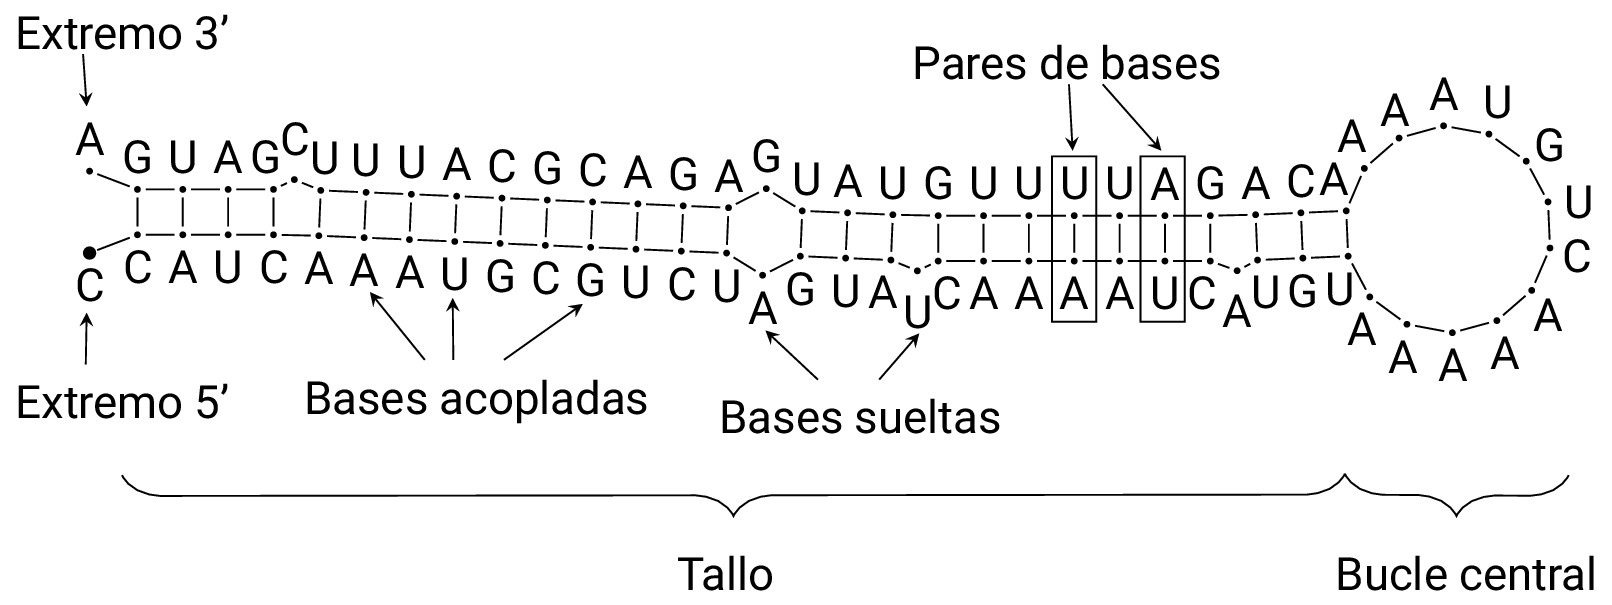
\includegraphics[width=.8\textwidth]{figures/hairpin_cel-lsy-6/hairpin.pdf}
%nnodes = 85
\shorthandoff{<}
\shorthandoff{>}
\tikzsetnextfilename{figures/hairpin_cel-lsy-6/hairpin}
\begin{tikzpicture}[scale=0.025,rotate=90,font=\small\sffamily,every label/.style={label distance=0}]
\tikzstyle{lstyle}=[shorten >= 2,shorten <= 2];
\coordinate[label={[xshift=0,yshift=0]below:C}] (1) at (93.0263,323.2249);
\fill[] (1) circle (2.2);
\coordinate[label={[xshift=0,yshift=0]below:C}] (2) at (99.0726,307.3858);
\fill[] (2) circle (1.1);
\coordinate[label={[xshift=0,yshift=0]below:A}] (3) at (99.0726,292.3858);
\fill[] (3) circle (1.1);
\coordinate[label={[xshift=0,yshift=0]below:U}] (4) at (99.0726,277.3858);
\fill[] (4) circle (1.1);
\coordinate[label={[xshift=0,yshift=0]below:C}] (5) at (99.0726,262.3858);
\fill[] (5) circle (1.1);
\coordinate[label={[xshift=0,yshift=0]below:A}] (6) at (98.7542,247.3892);
\fill[] (6) circle (1.1);
\coordinate[label={[xshift=0,yshift=0]below:A}] (7) at (98.1176,232.4027);
\fill[] (7) circle (1.1);
\coordinate[label={[xshift=0,yshift=0]below:A}] (8) at (97.4810,217.4162);
\fill[] (8) circle (1.1);
\coordinate[label={[xshift=0,yshift=0]below:U}] (9) at (96.8444,202.4297);
\fill[] (9) circle (1.1);
\coordinate[label={[xshift=0,yshift=0]below:G}] (10) at (96.2078,187.4432);
\fill[] (10) circle (1.1);
\coordinate[label={[xshift=0,yshift=0]below:C}] (11) at (95.5712,172.4568);
\fill[] (11) circle (1.1);
\coordinate[label={[xshift=0,yshift=0]below:G}] (12) at (94.9345,157.4703);
\fill[] (12) circle (1.1);
\coordinate[label={[xshift=0,yshift=0]below:U}] (13) at (94.2979,142.4838);
\fill[] (13) circle (1.1);
\coordinate[label={[xshift=0,yshift=0]below:C}] (14) at (93.6613,127.4973);
\fill[] (14) circle (1.1);
\coordinate[label={[xshift=0,yshift=0]below:U}] (15) at (93.0247,112.5108);
\fill[] (15) circle (1.1);
\coordinate[label={[xshift=0,yshift=0]below:A}] (16) at (85.6890,100.6079);
\fill[] (16) circle (1.1);
\coordinate[label={[xshift=0,yshift=0]below:G}] (17) at (91.9888,88.1258);
\fill[] (17) circle (1.1);
\coordinate[label={[xshift=0,yshift=0]below:U}] (18) at (91.3522,73.1393);
\fill[] (18) circle (1.1);
\coordinate[label={[xshift=-2,yshift=0]below:A}] (19) at (90.7156,58.1528);
\fill[] (19) circle (1.1);
\coordinate[label={[xshift=0,yshift=-2]below:U}] (20) at (87.1365,49.4132);
\fill[] (20) circle (1.1);
\coordinate[label={[xshift=2,yshift=0]below:C}] (21) at (90.3837,42.5196);
\fill[] (21) circle (1.1);
\coordinate[label={[xshift=0,yshift=0]below:A}] (22) at (90.3837,27.5196);
\fill[] (22) circle (1.1);
\coordinate[label={[xshift=2,yshift=0]below:A}] (23) at (90.3837,12.5196);
\fill[] (23) circle (1.1);
\coordinate[label={[xshift=0,yshift=0]below:A}] (24) at (90.3837,-2.4804);
\fill[] (24) circle (1.1);
\coordinate[label={[xshift=0,yshift=0]below:A}] (25) at (90.3837,-17.4804);
\fill[] (25) circle (1.1);
\coordinate[label={[xshift=0,yshift=0]below:U}] (26) at (90.3837,-32.4804);
\fill[] (26) circle (1.1);
\coordinate[label={[xshift=-2,yshift=0]below:C}] (27) at (90.3837,-47.4804);
\fill[] (27) circle (1.1);
\coordinate[label={[xshift=0,yshift=-2]below:A}] (28) at (87.1788,-56.3641);
\fill[] (28) circle (1.1);
\coordinate[label={[xshift=2,yshift=0]below:U}] (29) at (90.7156,-63.1136);
\fill[] (29) circle (1.1);
\coordinate[label={[xshift=0,yshift=0]below:G}] (30) at (91.3522,-78.1001);
\fill[] (30) circle (1.1);
\coordinate[label={[xshift=-2,yshift=0]below:U}] (31) at (91.9888,-93.0866);
\fill[] (31) circle (1.1);
\coordinate[label={[xshift=-2,yshift=0]below:A}] (32) at (78.5065,-100.2412);
\fill[] (32) circle (1.1);
\coordinate[label={[xshift=-1,yshift=0]below:A}] (33) at (69.4705,-112.5422);
\fill[] (33) circle (1.1);
\coordinate[label={[xshift=0,yshift=0]below:A}] (34) at (66.6749,-127.5471);
\fill[] (34) circle (1.1);
\coordinate[label={[xshift=2,yshift=0]below:A}] (35) at (70.6749,-142.2768);
\fill[] (35) circle (1.1);
\coordinate[label={[xshift=4,yshift=2]below:A}] (36) at (80.6762,-153.8066);
\fill[] (36) circle (1.1);
\coordinate[label={[xshift=-1,yshift=-2]right:C}] (37) at (94.6931,-159.8473);
\fill[] (37) circle (1.1);
\coordinate[label={[xshift=0,yshift=0]right:U}] (38) at (109.9425,-159.1995);
\fill[] (38) circle (1.1);
\coordinate[label={[xshift=-2,yshift=4]right:G}] (39) at (123.3966,-151.9918);
\fill[] (39) circle (1.1);
\coordinate[label={[xshift=2,yshift=0]above:U}] (40) at (132.3840,-139.6554);
\fill[] (40) circle (1.1);
\coordinate[label={[xshift=0,yshift=0]above:A}] (41) at (135.1205,-124.6396);
\fill[] (41) circle (1.1);
\coordinate[label={[xshift=0,yshift=0]above:A}] (42) at (131.0625,-109.9258);
\fill[] (42) circle (1.1);
\coordinate[label={[xshift=0,yshift=0]above:A}] (43) at (121.0159,-98.4354);
\fill[] (43) circle (1.1);
\coordinate[label={[xshift=0,yshift=0]above:A}] (44) at (106.9753,-92.4500);
\fill[] (44) circle (1.1);
\coordinate[label={[xshift=0,yshift=0]above:C}] (45) at (106.3387,-77.4635);
\fill[] (45) circle (1.1);
\coordinate[label={[xshift=0,yshift=0]above:A}] (46) at (105.7021,-62.4770);
\fill[] (46) circle (1.1);
\coordinate[label={[xshift=0,yshift=0]above:G}] (47) at (105.3837,-47.4804);
\fill[] (47) circle (1.1);
\coordinate[label={[xshift=0,yshift=0]above:A}] (48) at (105.3837,-32.4804);
\fill[] (48) circle (1.1);
\coordinate[label={[xshift=0,yshift=0]above:U}] (49) at (105.3837,-17.4804);
\fill[] (49) circle (1.1);
\coordinate[label={[xshift=0,yshift=0]above:U}] (50) at (105.3837,-2.4804);
\fill[] (50) circle (1.1);
\coordinate[label={[xshift=0,yshift=0]above:U}] (51) at (105.3837,12.5196);
\fill[] (51) circle (1.1);
\coordinate[label={[xshift=0,yshift=0]above:U}] (52) at (105.3837,27.5196);
\fill[] (52) circle (1.1);
\coordinate[label={[xshift=0,yshift=0]above:G}] (53) at (105.3837,42.5196);
\fill[] (53) circle (1.1);
\coordinate[label={[xshift=0,yshift=0]above:U}] (54) at (105.7021,57.5162);
\fill[] (54) circle (1.1);
\coordinate[label={[xshift=0,yshift=0]above:A}] (55) at (106.3387,72.5027);
\fill[] (55) circle (1.1);
\coordinate[label={[xshift=0,yshift=0]above:U}] (56) at (106.9753,87.4892);
\fill[] (56) circle (1.1);
\coordinate[label={[xshift=0,yshift=0]above:G}] (57) at (114.3110,99.3921);
\fill[] (57) circle (1.1);
\coordinate[label={[xshift=0,yshift=0]above:A}] (58) at (108.0112,111.8742);
\fill[] (58) circle (1.1);
\coordinate[label={[xshift=0,yshift=0]above:G}] (59) at (108.6478,126.8607);
\fill[] (59) circle (1.1);
\coordinate[label={[xshift=0,yshift=0]above:A}] (60) at (109.2844,141.8472);
\fill[] (60) circle (1.1);
\coordinate[label={[xshift=0,yshift=0]above:C}] (61) at (109.9210,156.8336);
\fill[] (61) circle (1.1);
\coordinate[label={[xshift=0,yshift=0]above:G}] (62) at (110.5576,171.8201);
\fill[] (62) circle (1.1);
\coordinate[label={[xshift=0,yshift=0]above:C}] (63) at (111.1943,186.8066);
\fill[] (63) circle (1.1);
\coordinate[label={[xshift=0,yshift=0]above:A}] (64) at (111.8309,201.7931);
\fill[] (64) circle (1.1);
\coordinate[label={[xshift=0,yshift=0]above:U}] (65) at (112.4675,216.7796);
\fill[] (65) circle (1.1);
\coordinate[label={[xshift=0,yshift=0]above:U}] (66) at (113.1041,231.7661);
\fill[] (66) circle (1.1);
\coordinate[label={[xshift=0,yshift=0]above:U}] (67) at (113.7407,246.7525);
\fill[] (67) circle (1.1);
\coordinate[label={[xshift=0,yshift=0]above:C}] (68) at (117.3198,255.4922);
\fill[] (68) circle (1.1);
\coordinate[label={[xshift=0,yshift=0]above:G}] (69) at (114.0726,262.3858);
\fill[] (69) circle (1.1);
\coordinate[label={[xshift=0,yshift=0]above:A}] (70) at (114.0726,277.3858);
\fill[] (70) circle (1.1);
\coordinate[label={[xshift=0,yshift=0]above:U}] (71) at (114.0726,292.3858);
\fill[] (71) circle (1.1);
\coordinate[label={[xshift=0,yshift=0]above:G}] (72) at (114.0726,307.3858);
\fill[] (72) circle (1.1);
\coordinate[label={[xshift=0,yshift=0]above:A}] (73) at (120.1190,323.2249);
\fill[] (73) circle (1.1);
\draw[lstyle] (1) -- (2);
\draw[lstyle] (2) -- (3);
\draw[lstyle] (3) -- (4);
\draw[lstyle] (4) -- (5);
\draw[lstyle] (5) -- (6);
\draw[lstyle] (6) -- (7);
\draw[lstyle] (7) -- (8);
\draw[lstyle] (8) -- (9);
\draw[lstyle] (9) -- (10);
\draw[lstyle] (10) -- (11);
\draw[lstyle] (11) -- (12);
\draw[lstyle] (12) -- (13);
\draw[lstyle] (13) -- (14);
\draw[lstyle] (14) -- (15);
\draw[lstyle] (15) -- (16);
\draw[lstyle] (16) -- (17);
\draw[lstyle] (17) -- (18);
\draw[lstyle] (18) -- (19);
\draw[lstyle] (19) -- (20);
\draw[lstyle] (20) -- (21);
\draw[lstyle] (21) -- (22);
\draw[lstyle] (22) -- (23);
\draw[lstyle] (23) -- (24);
\draw[lstyle] (24) -- (25);
\draw[lstyle] (25) -- (26);
\draw[lstyle] (26) -- (27);
\draw[lstyle] (27) -- (28);
\draw[lstyle] (28) -- (29);
\draw[lstyle] (29) -- (30);
\draw[lstyle] (30) -- (31);
\draw[lstyle] (31) -- (32);
\draw[lstyle] (32) -- (33);
\draw[lstyle] (33) -- (34);
\draw[lstyle] (34) -- (35);
\draw[lstyle] (35) -- (36);
\draw[lstyle] (36) -- (37);
\draw[lstyle] (37) -- (38);
\draw[lstyle] (38) -- (39);
\draw[lstyle] (39) -- (40);
\draw[lstyle] (40) -- (41);
\draw[lstyle] (41) -- (42);
\draw[lstyle] (42) -- (43);
\draw[lstyle] (43) -- (44);
\draw[lstyle] (44) -- (45);
\draw[lstyle] (45) -- (46);
\draw[lstyle] (46) -- (47);
\draw[lstyle] (47) -- (48);
\draw[lstyle] (48) -- (49);
\draw[lstyle] (49) -- (50);
\draw[lstyle] (50) -- (51);
\draw[lstyle] (51) -- (52);
\draw[lstyle] (52) -- (53);
\draw[lstyle] (53) -- (54);
\draw[lstyle] (54) -- (55);
\draw[lstyle] (55) -- (56);
\draw[lstyle] (56) -- (57);
\draw[lstyle] (57) -- (58);
\draw[lstyle] (58) -- (59);
\draw[lstyle] (59) -- (60);
\draw[lstyle] (60) -- (61);
\draw[lstyle] (61) -- (62);
\draw[lstyle] (62) -- (63);
\draw[lstyle] (63) -- (64);
\draw[lstyle] (64) -- (65);
\draw[lstyle] (65) -- (66);
\draw[lstyle] (66) -- (67);
\draw[lstyle] (67) -- (68);
\draw[lstyle] (68) -- (69);
\draw[lstyle] (69) -- (70);
\draw[lstyle] (70) -- (71);
\draw[lstyle] (71) -- (72);
\draw[lstyle] (72) -- (73);
\draw[lstyle] (2) -- (72);
\draw[lstyle] (3) -- (71);
\draw[lstyle] (4) -- (70);
\draw[lstyle] (5) -- (69);
\draw[lstyle] (6) -- (67);
\draw[lstyle] (7) -- (66);
\draw[lstyle] (8) -- (65);
\draw[lstyle] (9) -- (64);
\draw[lstyle] (10) -- (63);
\draw[lstyle] (11) -- (62);
\draw[lstyle] (12) -- (61);
\draw[lstyle] (13) -- (60);
\draw[lstyle] (14) -- (59);
\draw[lstyle] (15) -- (58);
\draw[lstyle] (17) -- (56);
\draw[lstyle] (18) -- (55);
\draw[lstyle] (19) -- (54);
\draw[lstyle] (21) -- (53);
\draw[lstyle] (22) -- (52);
\draw[lstyle] (23) -- (51);
\draw[lstyle] (24) -- (50);
\draw[lstyle] (25) -- (49);
\draw[lstyle] (26) -- (48);
\draw[lstyle] (27) -- (47);
\draw[lstyle] (29) -- (46);
\draw[lstyle] (30) -- (45);
\draw[lstyle] (31) -- (44);

%%%%%%%%%%%%%%%%

\usetikzlibrary{decorations.pathreplacing};
\coordinate (stemloop) at (20,-92);
\draw[decorate,decoration={brace, amplitude=10}] (stemloop)
to node [midway, label={[label distance=-20,below]:Tallo}] {} (20,320);
\draw[decorate,decoration={brace, amplitude=10}] (20,-170)
to node [midway, label={[label distance=-20,below]:Bucle central}] {} (stemloop);

\node (loose) at (40,70) {Bases sueltas};
\node (paired) at (45,200) {Bases acopladas};
\draw[-stealth] (loose) -- (70,50);
\draw[-stealth] (loose) -- (70,100);
\draw[-stealth] (paired) -- (80,160);
\draw[-stealth] (paired) -- (82,200);
\draw[-stealth] (paired) -- (84,230);

\draw[dotted] (73,-10) rectangle (125,6);
\draw[dotted] (73,-40) rectangle (125,-24);
\node (par) at (160,00) {Pares de bases};
\draw[-stealth] (par) -- (130,-2);
\draw[-stealth] (par) -- (130,-32);

\node (e5) at (45,320) {Extremo 5'};
\node (e3) at (170,320) {Extremo 3'};
\draw[-stealth] (e5) -- (75,330);
\draw[-stealth] (e3) -- (145,330);


\end{tikzpicture}
\shorthandon{<}
\shorthandon{>}


\caption{\captionStyle\protect\label{fig:hairpin-parts} Nomenclatura de las diferentes partes que
componen una la estructura secundaria típica en forma de horquilla.
El ejemplo corresponde a \protect\dset{lsy-6}, un \premirna{} de la
especie \e{C. elegans}, extraído de \work\mirbase{} versión 21.
}
\end{figure}
%
% esta footnote corresponde a la figura hairpin
\footnotetext{Fuente: \url{http://mirbase.org/cgi-bin/mirna_entry.pl?acc=MI0000801}.}
%
%
%
\subsubsection{Características de tripletes}
%
Las \caract{s} de tripletes, propuestas en el método \work{Triplet-SVM}
\cite{xue}, se basan en la idea de que la propiedad distintiva de los
\premirna{s} es una estructura secundaria en forma de horquilla
con una alta complementariedad entre las bases que forman el \e{tallo}.
%% En el trabajo original, los autores proponen un método para clasificar
%% secuencias con estructura secundaria en forma de horquilla entrenando
%% con \premirna{s} ``reales'' y otras secuencias con la misma estructura
%% secundaria denominadas ``pseudo \premirna{s}''.
Esta idea surge a partir de observar que la distribución
(frecuencia de aparición) de unas sub-estructuras locales llamadas
``tripletes'' difiere significativamente entre los ejemplos que
representan \premirna{s} y los ejemplos de otro tipo.

%% A partir de estas observaciones, proponen generar un conjunto de
%% \caract{s} que representa la distribución de las sub-estructuras
%% locales dentro del ``tallo'' de la horquilla.

Un ``triplete'' es una cadena de caracteres que relaciona la base de
un nucleótido (\ntA{}, \ntC{}, \ntG{}, o \ntU{}) en la posición $i$ con su
estructura secundaria local en $i-1,i,i+1$, representada en forma
binaria como ``acoplado'' \pairL{} (paréntesis) y ``no acoplado''
\noPair{} (punto).
El conjunto de \caract{s} de tripletes incluye medidas que cuentan
el número de ocurrencias de las $32$ combinaciones de tripletes posibles
($4$ bases $\cdot$ $2^3$ combinaciones de estado)
en la región del tallo, junto con $4$ medidas auxiliares que surgen
de cálculos intermedios:
%
\begin{itemize}
\item longitud del tallo $L_3$,
\item número de pares de bases $P$,
\item complementariedad de ambos brazos de la horquilla,
\item proporción de bases \ntG{} y \ntC{} en la zona del tallo.
\end{itemize}
%
En la \iflatexml{}Figura~\ref{triplet}\else\autoref{triplet}\fi{} se
representa en forma gráfica el proceso de extracción de las \caract{s}
de tripletes.

\begin{figure}[t]
\figureStyle
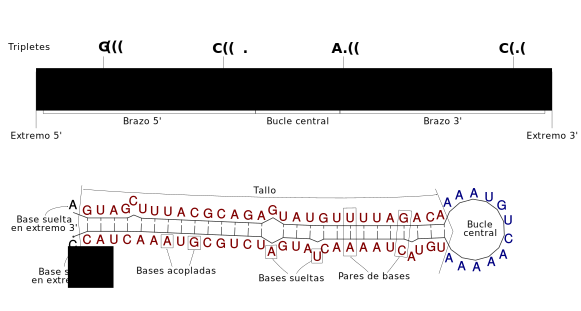
\includegraphics[width=\textwidth]{figures/triplet/triplete.pdf}

\caption{\captionStyle\protect\label{triplet}
Ejemplo de extracción de características de tripletes para el
\premirna{} \dset{cel-lsy-6}.
}
\end{figure}
%
%
\subsubsection{Características de tripletes}
%
Las \caract{s} de tripletes, propuestas en el método \work{Triplet-SVM}
\cite{xue}, se basan en la idea de que la propiedad distintiva de los
\premirna{s} es una estructura secundaria en forma de horquilla con
una alta complementariedad entre sus ``brazos''.
%% En el trabajo original, los autores proponen un método para clasificar
%% secuencias con estructura secundaria en forma de horquilla entrenando
%% con \premirna{s} ``reales'' y otras secuencias con la misma estructura
%% secundaria denominadas ``pseudo \premirna{s}''.
Las \caract{s} de tripletes se justifican en la observación empírica
que la distribución (frecuencia de aparición) de sub-estructuras
locales en la región del tallo de la horquilla difiere
significativamente entre los \premirna{s} ``reales'' y los ejemplos de
clase negativa, que también poseen estructura secundaria en forma de
horquilla.

%% A partir de estas observaciones, proponen generar un conjunto de
%% \caract{s} que representa la distribución de las sub-estructuras
%% locales dentro del ``tallo'' de la horquilla.

Un ``triplete'' es una cadena de caracteres que relaciona la base de
un nucleótido en la posición $i$ (\ntA, \ntC, \ntG, o \ntU) con su
estructura secundaria local en $i-1,i,i+1$, representada en forma
binaria como ``acoplado'' \pairL (paréntesis) y ``no acoplado''
\noPair (punto).
El conjunto de \caract{s} de tripletes incluye medidas que cuentan
el número de ocurrencias de las 32 combinaciones posibles de tripletes
en la región del tallo, junto con 4 medidas auxiliares derivadas
del cálculo de los tripletes:
%
\begin{itemize}
\item longitud del tallo,
\item número de pares de bases,
\item complementariedad de ambos brazos de la horquilla,
\item proporción de bases \ntG y \ntC en la zona del tallo.
\end{itemize}
%

En la \iflatexml{}Figura~\ref{triplet}\else\autoref{triplet}\fi{} se
ilustra el proceso de extracción de tripletes para el \premirna{}
\sbs{cel-lsy-66} correspondiente al organismo modelo \e{C. elegans}
\cite{mirbase1}, con anotaciones que indican las distintas partes que
componen la horquilla: tallo, bucle central, brazos, extremos, bases
sueltas y acopladas, y pares de bases.

La principal limitación de las características de tripletes reside en
que su cálculo resulta posible únicamente cuando la estructura
secundaria tiene forma de horquilla, ya que de otro modo la definición
del ``tallo'' pierde sentido. Por ello, estas \caract{s} no se
calculan cuando el ejemplo contiene bucles múltiples en su estrucutra
secundaria.

En la tabla a continuación se detallan las 36 características de
tripletes y su posición en el vector de características.

\newcommand{\tripletRow}[1]{
  \stepcounter{FeatureCounter}\theFeatureCounter &
  \dset{T} & $N_{\T{\mono{#1}}}$ &
  Número de ocurrencias del triplete \mono{#1} en la región del
  tallo. \iflatexml{}\\\fi
  }

\begin{longtable}{@{}p{0.07\textwidth}%
@{\hspace{0.01\textwidth}}p{0.07\textwidth}%
@{\hspace{0.01\textwidth}}p{0.13\textwidth}%
@{\hspace{0.01\textwidth}}p{0.70\textwidth}@{}}
  \headRow\endhead\iflatexml{}\\\fi
  \tripletRow{A...}\\
  \tripletRow{A..(}\\
  \tripletRow{A.(.}\\
  \tripletRow{A.((}\\
  \tripletRow{A(..}\\
  \tripletRow{A(.(}\\
  \tripletRow{A((.}\\
  \tripletRow{A(((}\\
  \tripletRow{G...}\\
  \tripletRow{G..(}\\
  \tripletRow{G.(.}\\
  \tripletRow{G.((}\\
  \tripletRow{G(..}\\
  \tripletRow{G(.(}\\
  \tripletRow{G((.}\\
  \tripletRow{G(((}\\
  \tripletRow{C...}\\
  \tripletRow{C..(}\\
  \tripletRow{C.(.}\\
  \tripletRow{C.((}\\
  \tripletRow{C(..}\\
  \tripletRow{C(.(}\\
  \tripletRow{C((.}\\
  \tripletRow{C(((}\\
  \tripletRow{U...}\\
  \tripletRow{U..(}\\
  \tripletRow{U.(.}\\
  \tripletRow{U.((}\\
  \tripletRow{U(..}\\
  \tripletRow{U(.(}\\
  \tripletRow{U((.}\\
  \tripletRow{U(((}\\
  33 & \dset{X} & $L_3$ &
  Longitud del tallo: cantidad de nucleótidos en el tallo de
  la estructura de horquilla. \\
  34 & \dset{X} & $P$ &
  Número de pares de bases en el \premirna{}. \\
  35 & \dset{X} & $L_3/P$ &
  Grado de complementariedad entre los dos brazos de la estructura de
  horquilla: para una complementariedad perfecta, se da el valor
  mínimo 2. Este valor aumenta conforme aumenta el número de
  bases ``sueltas'' (no acopladas) en el tallo. \\
  36 & \dset{X} & $GC=\frac{N_\ntC{}+N_\ntG{}}{L_3}$ &
  Proporción de bases \ntG{} y \ntC{} en el tallo.  Se calcula contando el
  número de bases \ntC{} y \ntG{} en el tallo y dividiendo por $L_3$.
\end{longtable}

%
%
\subsubsection{Características de la secuencia}
%
Las \caract{s} de la secuencia se proponen en los trabajos \e{miPred}
\cite{ng} y \e{microPred} \cite{batuwita}.
Estas \caract{s} se calculan directamente a partir de la secuencia,
ignorando las propiedades de la estructura secundaria.
Se incluyen medidas que cuentan la longitud de la secuencia, el número
de ocurrencias de las bases \ntA, \ntG, \ntC y\ntU en forma individual
y en combinaciones de dos posiciones consecutivas (dinucleótidos).
En la tabla a continuación se enumeran las 23 \caract{s} de la
secuencia según la posición que ocupan en el vector de \caract{s}.

\newcommand{\dnRow}[1]{
  \stepcounter{FeatureCounter}\theFeatureCounter
  & $N_{\T{\mono{#1}}}$
  & Número de dinucleótidos \mono{#1}.}
%
\setcounter{FeatureCounter}{43}
%
\begin{longtable}{@{}p{0.07\textwidth}%
@{\hspace{0.01\textwidth}}p{0.13\textwidth}%
@{\hspace{0.01\textwidth}}p{0.78\textwidth}@{}}
  \headRow\endhead
  37 & $L$ &
  Longitud de la secuencia. \\
  38 & $N_\ntA{}$ &
  Número de nucleótidos \ntA{}. \\
  39 & $N_\ntC{}$ &
  Número de nucleótidos \ntC{}. \\
  40 & $N_\ntG{}$ &
  Número de nucleótidos \ntG{}. \\
  41 & $N_\ntU{}$ &
  Número de nucleótidos \ntU{}. \\
  42 & $N_\ntC{}+N_\ntG{}$ &
  Número de nucleótidos \ntC{} y \ntG{}. \\
  43 & $N_\ntA{}+N_\ntU{}$ &
  Número de nucleótidos \ntA{} y \ntU{}. \\
  \dnRow{AA}\\
  \dnRow{AC}\\
  \dnRow{AG}\\
  \dnRow{AU}\\
  \dnRow{CA}\\
  \dnRow{CC}\\
  \dnRow{CG}\\
  \dnRow{CU}\\
  \dnRow{GA}\\
  \dnRow{GC}\\
  \dnRow{GG}\\
  \dnRow{GU}\\
  \dnRow{UA}\\
  \dnRow{UC}\\
  \dnRow{UG}\\
  \dnRow{UU}\\
\end{longtable}

%
%
\subsubsection{Características de la estructura secundaria}
%
Este grupo de \caract{s} incluye medidas relacionadas con la
estructura secundaria, tales como la ocurrencia de diferentes tipos de
pares de bases (bases acopladas) \bp{A}{U}, \bp{G}{C}, y \bp{G}{U}, así
como medidas basadas en la \e{Mínima Energía Libre}, un valor
resultante del algoritmo de plegado (predicción de la estructura
secundaria).  Al igual que las medidas de la secuencia, este grupo
de \caract{s} se basa en aquellas utilizadas en \cite{ng}
y \cite{batuwita}.  A continuación se detallan las 7 \caract{s} que
componen este grupo y su posición dentro del vector global
de \caract{s}.

\begin{longtable}{@{}p{0.07\textwidth}%
@{\hspace{0.01\textwidth}}p{0.07\textwidth}%
@{\hspace{0.01\textwidth}}p{0.13\textwidth}%
@{\hspace{0.01\textwidth}}p{0.70\textwidth}@{}}
  \headRow\endhead
  60 & \dset{E} & MFE &
  Mínima energía libre. \\
  61 & \dset{E} & MFEI$_1$ &
  MFEI$_1=\frac{\T{MFE}}{100\cdot(N_\ntC{}+N_\ntG{})}$. \\
  62 & \dset{E} & MFEI$_4$ &
  MFEI$_4=\T{MFE}/P$. \\
  63 & \dset{E} & $dP = P/L$ &
  Número de pares de bases dividido entre la longitud total $L$. \\
  64 & \dset{E} & $P_{\bp{A}{U}}/L$ &
  Número de pares \bp{A}{U} normalizado. \\
  65 & \dset{E} & $P_{\bp{G}{C}}/L$ &
  Número de pares \bp{G}{C} normalizado. \\
  66 & \dset{E} & $P_{\bp{G}{U}}/L$ &
  Número de pares \bp{G}{U} normalizado.
\end{longtable}

%
%
%
\subsection{Normalización de los vectores de características}
%
Las \caract{s} que componen el vector de \caract{s} poseen rangos
numéricos diferentes, ya que representan cantidades de naturaleza
diversa.
Esto implica que algunos componentes del vector de \caract{s} tendrán
magnitudes mayores que otros, generando una ponderación implícita de
algunas \caract{s} por sobre otras.
La normalización permite evitar este problema modificando el rango de
cada \caract{} a un intervalo preestablecido, típicamente $[0,1]$ o
$[-1,+1]$.
Esto deriva en problemas mejor condicionados desde el punto de vista
numérico e incrementa la velocidad de convergencia en el
entrenamiento \cite{nnfaq2}.

Dado un vector de características $\xx=(x_{1},x_{2},\ldots,x_{F})$, la
versión normalizada $\xx^*$ del mismo vector se calcula según
%
\begin{align}
  \label{e3:norm-op}
  x_j^{*} = ( x_j + d_j ) s_j, \quad j=1,\ldots,F,
\end{align}
%
donde $\B{s}$ es un \e{vector de escala} y $\B{d}$ es un \e{vector de
  desplazamiento} que permiten transformar las componentes $x_j$ al
intervalo especificado.

Cuando el objetivo es la generación de un modelo de clasificador, los
vectores $\B{s}$ y $\B{d}$ se calculan con el primer archivo leído a
la entrada del método.
El primer paso es armar una matriz
$M{}_{({N}\times{}F)}$, donde cada fila $i=1,\ldots,N$ corresponde a
un ejemplo y cada columna $j=1,\ldots,F$ representa una variable
(\caract{}).
Para cada columna $j$ de $M$, se calculan los valores $d_j$ y $s_j$
que transforman el rango de la variable $x_j$ al intervalo deseado.
Para llevar las variables al rango $[0,1]$, $d_j$ y $s_j$ se
calculan según
%
\begin{align}
  d_j &= - \min_i m_{ij}, &
  s_j &= \frac{1}{\max_i m_{ij} - \min_i m_{ij}}.
\end{align}
%
Similarmente, para llevar las variables al intervalo simétrico
$[-1,+1]$,
%
\begin{align}
  d_j &= -\frac{1}{2}\left(\max_i m_{ij} + \min_i m_{ij}\right), &
  s_j &= \frac{2}{\max_i m_{ij} - \min_i m_{ij}}.
\end{align}
%
Una vez calculados los vectores $\B{d}$ y $\B{s}$, se aplica la
normalización (\iflatexml{}Ecuación~\ref{e3:norm-op}\else\autoref{e3:norm-op}\fi)
sobre todos los ejemplos leídos en la entrada.

Para un modelo de clasificador entrenado con datos normalizados, es
importante aplicar la misma normalización sobre todos los ejemplos
futuros a clasificar.
Por ello, los vectores $\B{d}$ y $\B{s}$ se guardan como parte del
mismo modelo.
Cuando se provee un modelo como entrada al método, los ejemplos se
normalizan según la información contenida en el mismo.

%
%
%
\subsection{Particionado de los datos}
%
El particionado separa los datos leídos en conjuntos de entrenamiento,
utilizado para la generación del modelo del clasificador, y de prueba,
que contiene los ejemplos a usar para clasificación.
La composición de estos conjuntos viene determinada por la
especificación del usuario, que debe indicar, para cada archivo, el
número de elementos a utilizar para entrenamiento y para prueba.
Cuando el archivo se utiliza para entrenamiento, se debe indicar
adicionalmente la clase de los ejemplos que contiene.

El primer paso es ``etiquetar'' los vectores normalizados, extendiéndolos
con números de referencia que indican el archivo de origen, la
posición del dato original dentro del archivo, y la clase del ejemplo
en cuestión.
El segundo paso armar los conjuntos de entrenamiento y prueba como
matrices, cuyas filas son vectores ``etiquetados'' seleccionados al
azar de cada archivo, respetando las proporciones indicadas por el
usuario.
Una vez incorporados todos los ejemplos a los conjuntos de
entrenamiento y prueba, se permutan las filas de ambas matrices en
forma pseudoaleatoria.

La partición de los datos se efectúa de forma tal que los conjuntos de
entrenamiento y prueba resultantes sean disjuntos: si un ejemplo se
incorpora al conjunto de prueba, no será parte del conjunto de
entrenamiento, y viceversa.

%
%
\subsubsection{Generación de particiones para validación cruzada}
%
%La generación de las particiones de validación cruzada se lleva a cabo
%una vez armado el conjunto de entrenamiento con $\ell^E$ elementos.
Las particiones de validación cruzada se generan como un conjunto de
índices sobre el conjunto de entrenamiento.
En primer lugar, se genera un vector de índices en orden aleatorio
entre $1$ y $\ell^E$, el número de ejemplos en el conjunto de
entrenamiento.
Luego se seleccionan los primeros $p\cdot\ell^E$ elementos para la
partición de validación, y los elementos restantes para la partición
de estimación correspondiente.
La operación se repite para cada $j=1,\ldots,k$, efectuando un
desplazamiento circular del vector de índices en $\ell^E/k$ elementos
entre iteraciones.
El parámetro $p$ regula la proporción de elementos de entrenamiento a
utilizar para validación, mientras que $k$ determina el número de
iteraciones de la validación cruzada.
Ambos parámetros pueden ser especificados por el usuario, y por
defecto se utilizan los valores $k=10$ $p=1/$.
Cuando $p=1/k$, cada ejemplo del conjunto de entrenamiento será
utilizado exactamente una vez para validación.

%
%
%
\section{Construcción del modelo del clasificador MLP}
%
El primer paso para la construcción de un modelo MLP es determinar el
número óptimo de neuronas en la capa oculta mediante una estrategia
de búsqueda exhaustiva que maximiza la tasa \GM{} promedio de
validación cruzada.
%% Para ello, se utiliza una estrategia de prueba y error, que prueba
%% distintos modelos mediante validación cruzada, y selecciona como
%% número óptimo de neuronas el de aquel modelo que obtiene la mejor tasa
%% $G_m$ en promedio sobre el conjunto de validación.
Alternativamente, se define una estrategia de selección trivial que
siempre selecciona 0 neuronas en la capa oculta, resultando en un
clasificador lineal.

Una vez determinado el número óptimo de neuronas en la capa oculta,
se procede al entrenamiento del modelo final utilizando el conjunto
de entrenamiento completo.

%% uego se procede a efectuar el entrenamiento propiamente dicho, con
%% regularización de corte prematuro cuando el error de validación
%% cruzada alcanza su valor mínimo.

%% La arquitectura de la red resultante contendrá una o ninguna capa
%% oculta.

%% En todo entrenamiento del clasificador, se promedian en realidad cinco
%% redes inicializadas aleatoriamente, y la salida del clasificador en
%% realidad es un voto mayoritario de la salida de estas cinco redes.

%% Adicionalmente, se acepta el valor especial de 0 neuronas ocultas para
%% representar un MLP sin capa oculta, capaz de efectuar clasificación lineal.

%% Las estrategias de selección del \hparam{} de la red (el número de
%% neuronas en la capa oculta) son
%% %
%% \begin{description}
%% \item[Estrategia trivial:] Consiste en seleccionar cero neuronas
%%   en la capa oculta, sin entrenamiento. Esto redunda en una red que es
%%   capaz de efectuar separación lineal, y se utiliza como criterio de base para
%%   establecer el rendimiento de la red.
%% \item[Estrategia de búsqueda exhausiva:] Consiste en determinar, mediante prueba y error,
%%   el número óptimo de neuronas que maximizan una tasa promedio de validación cruzada.
%% \end{description}
%% %
%% Una vez encontrado el valor óptimo, se procede al entrenamiento.

%
\subsection{Estrategia trivial}
%
La estrategia trivial retorna siempre el valor 0 como cantidad
``óptima'' de neuronas en la capa oculta, ignorando los datos de
entrenamiento.
El modelo de clasificador MLP resultante del entrenamiento siempre
equivale a un perceptrón simple, que funciona como un clasificador
lineal.
Si bien resulta claro que esta estrategia no efectssss ningnnnn tipo
de optimización, su utilidad reside en que el modelo resultante puede
tomarse como base en la comparación de distintos modelos MLP para el
problema dado.
%
%% En el caso de las
%% máquinas de vectores de soporte, la estrategia selecciona el valor $1$
%% para el hiperparámetro de regularización $C$ \cite{libsvm}, y un valor
%% $\gamma=\frac{1}{2F}$ para el hiperparámetro de amplitud del núcleo
%% RBF, donde $F$ es el número de características consideradas
%% \cite{glasmachersigel}.
%

%
\subsection{Búsqueda exhaustiva}
%
La estrategia de búsqueda exhaustiva determina el número óptimo de
neuronas ocultas mediante prueba y error, entrenando modelos con
diferentes cantidades de neuronas en la capa oculta y seleccionando
aquel que obtiene la mayor tasa \GM{} de validación cruzada en
promedio.

Dado que no existe una regla general para determinar el número
recomendado de neuronas ocultas \cite{nnfaq3}, se establece un rango
de prueba de entre 0 y 200.
Por razones de costo computacional, en lugar de efectuar la búsqueda
sobre todos los valores posibles, se prueban 20 valores $h$ entre 0 y
200 en una escala aproximadamente logarítmica:
%
\begin{align}
  \label{mlp-hidden-tries}
  h=0,1,2,3,4,5,7,9,11,14,19,24,32,41,54,70,91,118,154,200.
\end{align}
%
%% La estrategia genera selecciona aquel valor de $h$ para el cual se obtuvo
%% el mayor \GM de validación cruzada en promedio.

%
\subsubsection{Entrenamiento}
%
Una vez determinados los hiperparámetros óptimos del clasificador
mediante alguna de las estrategias descriptas previamente, se entrena
una máquina de aprendizaje (SVM o MLP) con el conjunto de
entrenamiento completo $D$, obteniendo un modelo ``final''.

La salida del método consiste en el modelo de la máquina de
aprendizaje correspondiente, el cual servirá, junto a una
especificación del escalado y offset a utilizar, para clasificar
elementos nuevos.

Para el caso del perceptrón multicapa, el modelo en realidad
consiste en 5 redes neuronales inicializadas con datos aleatorios
y entrenadas con el mismo conjunto de datos $D$.
De este modo, se neutraliza hasta cierto punto los efectos negativos
que una red mal ondicionada pudiera generar un mal modelo.

{\Huge \hl{Agregar detalles implementacion pertinentes}}

%
%
\section{Construcción del modelo del clasificador SVM}
%
Tal como en el caso del perceptrón multicapa, la construcción del
modelo SVM es un proceso de dos etapas: en primer lugar se determinan
valores óptimos para los \hparam{s}, y una vez encontrados, se procede
a entrenar el modelo final con los datos de entrenamiento y los
\hparam{s} óptimos encontrados.
%% A diferencia del caso MLP, sin embargo, en una máquina de vectores de
%% soporte puede haber más de un \hparam{}, y en general éstos se trata
%% de variables continuas.

Las propiedades analíticas de la SVM permiten aplicar estrategias de
selección de hiperparámetros más complejas que en el caso del MLP, que
en general resultan computacionalmente más eficientes.
Las cuatro estrategias de selección de \hparam{s} aplicables al
clasificador SVM son:
%
\begin{itemize}
\item
  Selección trivial: Retorna valores preestablecidos para los
  \hparam{s}, sin efectuar entrenamiento.
\item
  Búsqueda en la grilla: Efectúa una búsqueda exhaustiva de los
  hiperparámetros, maximizando la tasa de clasificación de validación
  cruzada.
\item
  Minimización del error empírico: Minimiza, mediante descenso por
  gradiente en el espacio de los \hparam{s}, una función que representa
  el error de clasificación de validación cruzada.
\item
  Minimización de la cota radio-margen: Minimiza mediante descenso por
  gradiente en el espacio de los \hparam{s} una función de derivación
  teórica que se relaciona con el error de clasificación.
\end{itemize}
%

%
%
\subsection{Selección trivial}
%
La estrategia de selección trivial consiste en seleccionar valores
preestablecidos (genéricos) para los hiperparámetros, apropiados para
la mayoría de los problemas.
El valor preestablecido para el hiperparámetro de regularización $C$
es $1$ \cite{libsvm}.
En el caso del hiperparámetro de amplitud del núcleo RBF, se calcula
un valor $\gamma=\frac{1}{2F}$, donde $F$ es el número de elementos en
el vector de características \cite{glasmachersigel}.

Es de esperar que el modelo resultante del uso de esta estrategia no
sea óptimo, aunque sí resulta de utilidad como base para la
comparación contra otros modelos parametrizados con estrategias más
complejas.

%
%
\subsection{Búsqueda en la grilla}
%
La \e{búsqueda en la grilla} es una estrategia heurística basada en el
método propuesto en \cite{hsu} que calcula valores óptimos para los
\hparam{s} de regularización $C$ y de amplitud del núcleo RBF
$\gamma$.
La estrategia considera las combinaciones de $(C,\gamma)$ como
``coordenadas en el espacio de los \hparam{s}''.
En cada punto $(C,\gamma)$, se entrena el clasificador con los
\hparam{s} correspondientes y se evalúa el resultado de validación
cruzada.
La búsqueda comienza con una ``grilla'' de puntos espaciados a
intervalos regulares y continúa interpolando en las cercanías de
aquellos puntos donde se obtuvo las mayores tasas de clasificación de
validación cruzada.

La grilla inicial viene dada por las coordenadas $C$-$\gamma$
%
\begin{align}
  \label{initial-grid}
  \log_2 C     \tab= -5, -3, -1, 1, \ldots, 15, \tabs
  \log_2\gamma \tab= -15,-13, -11, \ldots, 3.
\end{align}
%
Para cada punto $(C_i,\gamma_j)$, se entrena un modelo con los
\hparam{s} correspondientes y se clasifican las particiones de
validación cruzada, obteniendo una tasa $\GM_{ij}$ promedio.

La interpolación de la grilla se lleva a cabo mediante alguno de los
siguientes algoritmos heurísticos:
%
\begin{itemize}
\item
  \e{Zoom}: interpola una región centrada en el punto con mayor tasa
  de clasificación, reduciendo el área de búsqueda a $1/2$ de la
  amplitud anterior en cada dimensión.
\item
  \e{Umbral}: interpola puntos intermedios alrededor de las
  coordenadas cuyo resultado se ubica por encima de un valor
  ``umbral'', por defecto el percentil 90 de toda la grilla.
  Este algoritmo es el utilizado por defecto.
\item
  \e{$n$-mejores}: similar al umbral, interpola la grilla alrededor de
  los $n$ puntos con mejores resultados de validación cruzada.
\end{itemize}
%
Luego de efectuar la interpolación, se entrena y prueba el
clasificador sobre los nuevos puntos generados.
El procedimiento se repite $N$ iteraciones (por defecto, $N=3$).

La búsqueda en la grilla tiene la ventaja de ser conceptualmente
simple, sin embargo, no resulta escalable a más de dos dimensiones.
Dado que se trata de un método de búsqueda exhaustiva, resulta
comparativamente lento.
Cuando se trabaja con un clasificador SVM con núcleo lineal, se
establece la coordenada $\gamma=0$, y la grilla resultante tiene una
única dimensión, la del hiperparámetro $\log C$.

%
%
\subsection{Criterio del error empírico}
%
El \e{criterio del error empírico} es una estrategia que optimiza los
\hparam{s} del clasificador minimizando una función objetivo
denominada \e{error empírico}\,\footnote{
  El lector experto encontrará ambigua la denominación de la función
  ``error empírico'', ya que en la disciplina este nombre se utiliza
  como equivalente de ``error de entrenamiento''.
  En este trabajo, se mantiene la denominación de los autores
  \cite{ayat}, definiendo ``error empírico'' como la función que
  calcula un error probabilístico de validación cruzada sobre el
  conjunto de entrenamiento.
}, basada en la propuesta presentada en \cite{ayat}.
La función de error empírico mide el error de validación cruzada sobre
el conjunto de entrenamiento acoplando un modelo probabilístico a la
salida del clasificador, y permite su optimización mediante descenso
por gradiente ya que sus derivadas respecto de los \hparam{s} son
calculables.

En la propuesta original \cite{ayat}, la función {error empírico} se
optimiza únicamente respecto a los \hparam{s} del núcleo.
En la estrategia implementada, se agregó soporte para la optimización
del hiperparámetro $C$, siguiendo el método del cálculo de la derivada
respecto de $C$ propuesto en \cite{keerthi} y \cite{glasmachers}, tal
como se implementa en \cite{shark}.

%
\subsubsection{La función error empírico}
%
La función error empírico es la función objetivo a minimizar, y se
construye a partir de una estimación de la probabilidad de error del
modelo sobre el conjunto de entrenamiento.
Esta función posee características deseables de continuidad y
derivabilidad que permiten su optimización mediante descenso por
gradiente.

Considerando en primer lugar la pérdida $0-1$ promedio del modelo $h$
sobre un conjunto de validación $V=((\xx_k,y_k)),\,i=1,\ldots,\ell^V$,
se observa que este error puede escribirse
%
\begin{align}
\label{e3:error-test-alt}
E^V \tab = \frac{1}{\ell^V}\sum_{k=1}^{\ell^V} H(-{y}_k {h}(\xx_k))
\tabs = \frac{1}{\ell^V}\sum_{k=1}^{\ell^V} L_{0-1}(y_k,h(\xx_k)).
\end{align}
%
El uso de la función escalón unitario de Heaviside $H(\cdot)$ pone de
relieve el hecho que $E^V$ es una suma de funciones discontinuas, y
por lo tanto no es derivable.
Para salvar esta limitación, la función error empírico se construye a
partir de una estimación $\hat{p}_k$ de la \e{probabilidad a
  posteriori} $p_k$ de que el ejemplo $\xx_k$ pertenezca a la clase
positiva
%
\begin{align}
  \label{e3:pk}
  p_k = p(\xx_k) = P(h(\xx_k)=+1|\xx_k).
\end{align}
%
Por el momento, se supone que $p_k$ es una función continua y
derivable.
La \e{probabilidad de error} $E_k$ del modelo al clasificar el ejemplo
$\xx_k$ puede escribirse en términos de la probabilidad $p_k$ según
%
\begin{align}
\label{e3:Ek}
  E_k = P(h(\xx_k)\neq y_k) = |t_k-{p}_k| =
  \begin{cases}
    {p}_k, & t_k=0\\ 1-{p}_k, & t_k = 1,
  \end{cases}
\end{align}
%
en donde $t_k=\frac{1}{2}({y_k+1})$ es un ``valor deseado'' calculado
a partir de la clase conocida $y_k$.
El error empírico es simplemente la probabilidad de error promedio
para el conjunto completo $V$:
%
\begin{align}
\label{Err1}
  E = \frac{1}{\ell^V}\sum_{j=1}^{\ell^V} E_k.
\end{align}
%
Para el cálculo exacto de $E$ se requiere conocer la probabilidad
$p_k$ (\iflatexml{}Ecuación~\ref{e3:pk}\else\autoref{e3:pk}\fi), la
cual no puede determinarse a partir de la salida binaria del modelo
SVM.
En su lugar se utiliza un estimador $\hat{p}_k$, que se obtiene
ajustando un modelo probabilístico a la salida del modelo, tal como se
explica a continuación.

%
\subsubsection{Salida probabilística del modelo SVM}
%
La salida del modelo de una \MVS{} (\ref{e2:svm-model-hard}) puede
entenderse como el resultado de aplicar la operación signo sobre una
función continua $f$:
%
\begin{align}
\label{e3:svm-model-as-sign-f}
  h(\xx) \tab= \T{signo}(f),\tabs
  f\tab=\pint{\ww}{\BPhi(\xx)}+b.
\end{align}
%
Aplicando el método propuesto por {Platt} en \cite{platt}, se calcula
un estimador $\hat{p}$ para la probabilidad real $p=P(h=+1|\xx)$
utilizando el valor de $f$:
%
\begin{align}
\label{e3:p-hat}
  \hat{p}\tab=\frac{1}{1+e^{Af+B}} \tabs\approx\,{}p.%P(h=+1|\xx).
\end{align}
%
Los valores $A$ y $B$ se determinan a partir de un conjunto de validación
$V$ resolviendo el problema de optimización
%
\begin{align}
  \arg\min_{A,B} \tabs -\sum_{j=1}^{\ell^V} t_k\log(\hat{p}_k)+(1-t_k)\log(1-\hat{p}_k),
  \label{abproblem}
\end{align}
%
en donde $\hat{p}_k$ viene dado por (\ref{e3:p-hat}), y
$t_k=\frac{1}{2}({y_k+1})$.
Este problema se resuelve mediante el algoritmo de optimización
estándar BFGS \cite{nocedal}, observando que las derivadas de
$\hat{p}_k$ respecto de $A$ y $B$ vienen dadas por
%
\begin{align}
  \begin{split}
    \dpar{\hat{p}_k}{A}{}&=-f_k e^{Af_k+B}\frac{1}{(1+e^{Af_k+B})^2}
    =-f_k\hat{p}_k(1-\hat{p}_k),\\
    \dpar{\hat{p}_k}{B}{}&=    -e^{Af_k+B}\frac{1}{(1+e^{Af_k+B})^2}
    =-   \hat{p}_k(1-\hat{p}_k).
  \end{split}
\label{e3:deriv-pk-wrt-AB}
\end{align}
%
%% Utilizando estas derivadas, el cálculo de la solución al problema
%% (\ref{abproblem}) se efectúa mediante un algoritmo de descenso por
%% gradiente.

%% La elección de una función logística como $\hat{p}_k$ se basa en la
%% presunción de que las salidas $f_k$ para las entradas $\{\xx_k\}$ de
%% clase positiva tienen una distribución gaussiana en $f$.

%% Una interpretación intuitiva de $\hat{p}_k$ es que, para una salida
%% $f_k$ de gran magnitud, que se ubica lejos del hiperplano de separación
%% en el espacio inducido por el núcleo, el clasificador SVM tiene amplia
%% certeza de su decisión.  Asimismo, se tendrá que cuando el valor de
%% $f_k=0$, $x_k$ recae exactamente en el plano de separación y se
%% obtiene la peor predicción posible $\hat{p}_k=0.5$ y, similarmente,
%% cuanto más ancho sea el margen de separación, más suave deberá ser la
%% pendiente de $\hat{p}_k$.

%
\subsubsection{Cálculo del gradiente $\grad{E}$}
\label{se:gradE}
%
Considerando un vector genérico de \hparam{s}
$\Btheta=(\theta_1,\theta_2,\ldots)$, el gradiente
$\nabla{}E=\left(\dpar{E}{\theta}{}\right)$ se calcula según
%
\begin{align}
\label{gradE}
  \dpar{E}{\theta_j}{} = \sum_{k=1}^{\ell^V} \dpar{E_k}{\theta_j}{} =
  \sum_{ \{m:t_k=0\}  } \dpar{\hat{p}_m}{\theta_j}{}
  - \sum_{ \{n:t_k=1\}  } \dpar{\hat{p}_n}{\theta_j}{}
  = \sum_{k=1}^{\ell^V} y_k \dpar{\hat{p}_k}{\theta_j}{}.
\end{align}
%
Aplicando la regla de la cadena y calculando la derivada
$\dpar{\hat{p}_k}{f_k}{}$, se tiene
%
\begin{align}
  \dpar{\hat{p}_k}{\theta_j}{} =
  \dpar{\hat{p}_k}{f_k}{}\dpar{f_k}{\theta_j}{} =
  -A\hat{p}_k(1-\hat{p}_k)\dpar{f_k}{\theta_j}{}.
  \label{eq:deriv-pk-thetaj}
\end{align}
%
Para el cálculo de $\dpar{f_k}{\theta_j}{}$ a continuación se recurre
a una interpretación geométrica del modelo SVM con regularización $L1$
tal como en \cite{keerthi,glasmachers,shark}.
En primer lugar, se observa que $f_k$ viene dado por
%
\begin{align}
  f_k = \langle \ww,\Phi(\xx_k)\rangle+b
      = \sum_{i=1}^\ell \alpha_i y_i k(\xx_i,\xx_k) + b,
  \label{fk}
\end{align}
%
en donde $((\xx_i,y_i)),\,i=1,\ldots,\ell$ son los ejemplos del
conjunto utilizado para entrenamiento, $k(\cdot,\cdot)$ es la función
núcleo, y $(\alpha_i, b)$ son los parámetros del modelo SVM $h$.
Aplicando la regla de la derivada de un producto,
$\dpar{f_k}{\theta_j}{}$ viene dada por
%g
\begin{align}
  \dpar{f_k}{\theta_j}{} = \sum_{i=1}^\ell y_i
  \left[\dpar{\alpha_i}{\theta_j}{} k(\xx_i,\xx_k) + \alpha_i
    \dpar{k(\xx_i,\xx_k)}{\theta_j}{} \right].
\end{align}
%
Según sea el valor de $\alpha_i$, el multiplicador correspondiente al
vector de entrenamiento $\xx_i$, se definen los conjuntos de índices
%
\begin{align}
  \label{unbounded-sv-set}
  u &= \left\{i\in\{1,\ldots,\ell\}:0<y_i\alpha_i<C \right\}\\
  \label{bounded-sv-set}
  g &= \left\{i\in\{1,\ldots,\ell\}: y_i\alpha_i=C \right\}\\
  n &= \left\{i\in\{1,\ldots,\ell\}: \alpha_i=0 \right\}.
\end{align}
%
Efectuando una interpretación geométrica de la solución al problema de
la SVM (\iflatexml{}Ecuación~\ref{svmprob-dual-soft}\else\autoref{svmprob-dual-soft}\fi),
se sabe que para aquellos vectores $\xx_i$ que no son de soporte, se
cumple que $\alpha_i=0$, luego las derivadas
$\dpar{\alpha_n}{\theta_j}{}$ son nulas.
Cuando $\alpha_i=\pm{}C$, el valor de $\alpha_g$ viene limitado (en
valor absoluto) por el \hparam{} $C$, y las derivadas
$\dpar{\alpha_g}{\theta_j}{}$ son entonces
%
\begin{align}
  \dpar{\alpha_g}{C}{} \tab= y_g, \tabs
  \dpar{\alpha_g}{{\theta}^K_j}{} \tab= 0,
\end{align}
%
en donde $\theta_j^K$ es un hiperparámetro del núcleo.
Para simplificar el cálculo de las derivadas de $\alpha_u$ y $b$, se
plantea el problema en forma matricial.
Se plantea entonces la \e{matriz del núcleo} $K$
%
\begin{align}
  K = \begin{pmatrix} k(\xx_1,\xx_1) & k(\xx_1,\xx_2) & \cdots & k(\xx_1,\xx_\ell)
    \\ k(\xx_2,\xx_1) & k(\xx_2,\xx_2) & \cdots & k(\xx_2,\xx_\ell) \\ \vdots &
    \vdots & \ddots & \vdots \\ k(\xx_\ell,\xx_1) & k(\xx_\ell,\xx_2) & \cdots &
    k(\xx_\ell,\xx_\ell)
  \end{pmatrix}
  =
  \begin{pmatrix}
    (K_{uu}) & (K_{ug}) & (K_{un}) \\
    (K_{gu}) & (K_{gg}) & (K_{gn}) \\
    (K_{nu}) & (K_{ng}) & (K_{nn})
  \end{pmatrix}.
\end{align}
%
En la matriz de la derecha, los elementos de $K$ han sido reordenados
en submatrices $K_{uu},K_{ug},\ldots$ según los conjuntos de índices
$u, g, n$ definidos anteriormente.
Entonces, se calcula la matriz
%
\begin{align}
  H=\begin{pmatrix} K_{uu} & \B{1}_u \\ \B{1}_u^T & 0
  \end{pmatrix},
\end{align}
%
en donde $\B{1}_u$ es un vector columna de $|u|$ elementos iguales a 1.
La derivada de $(\B{\alpha}_u,b)^T$ respecto de un \hparam{}
$\theta_j$ viene dada por
%
\begin{align}
  \dpar{}{\theta^K_j}{} \begin{pmatrix}\alpha_{u}\\b\end{pmatrix} &=
    -H^{-1} \left[
      \dpar{H}{\theta^K_j}{}
      \begin{pmatrix}\alpha_{u}\\b\end{pmatrix}
        +C \begin{pmatrix}\dpar{K_{gu}}{\theta^K_j}{}\\0\end{pmatrix}
          y_g
          \right],
\end{align}
%
donde $\B{1}_g$ es un vector columna de $|g|$ elementos iguales a 1 y
$\B{y}_g$ es el vector de clases correspondientes a los elementos en
$g$.
Cuando $\theta_j = C$, se tiene
%
\begin{align}
  \dpar{}{C}{} \begin{pmatrix}\alpha_{u}\\b\end{pmatrix} &=
    -H^{-1} \left[
      \begin{pmatrix}{K_{gu}}\\\B{1_g^T}\end{pmatrix} y_g
      \right].
\end{align}
%
Para los detalles de este resultado, se refiere al lector a
\cite{glasmachers} y \cite{keerthi}.
Una vez conocidas las derivadas
$\dpar{({\B{\alpha},b})^T}{\theta_j}{}$, la derivada
$\dpar{f}{\theta_j}{}$ se calcula según
%
\begin{align}
  \dpar{f_k}{\theta^K_j}{} &=  \sum_{i=1}^l y_i \left[
    \dpar{\alpha_i}{\theta^K_j}{} k(x_i,x_k) +
    \dpar{k(x_i,x_k)}{\theta^K_j}{} \alpha_i \right]
  + \dpar{b}{\theta^K_j}{}, \\
    \dpar{f_k}{C}{} &=  \sum_{i=1}^l y_i\left[
    \dpar{\alpha_i}{C}{} k(x_i,x_k) \right]
  + \dpar{b}{C}{}.
\end{align}
%
Reemplazando estos resultados en la
\iflatexml{}Ecuación~\ref{eq:deriv-pk-thetaj}\else\autoref{eq:deriv-pk-thetaj}\fi{},
el gradiente $\nabla{}E=\left(\dpar{E}{\theta_j}{}\right)$
(\iflatexml{}Ecuación~\ref{gradE}\else\autoref{gradE}\fi{}) se calcula
directamente.

%
\subsubsection{Algoritmo de optimización}
%
Dado el conjunto de entrenamiento $D$, en cada punto de evaluación
$\Btheta$ el error empírico $E(\Btheta)$ se calcula del siguiente modo
%
\begin{enumerate}
\item
  Aplicando validación cruzada, se entrena un modelo SVM para cada
  conjunto de estimación.
\item
  Se calculan las salidas $f_k$
  (\iflatexml{}Ecuación~\ref{fk}\else\autoref{fk}\fi) de los modelos
  para todos los ejemplos $\xx_k$ en las respectivas particiones de
  validación.
\item
  Se determinan los valores óptimos de los parámetros $A$ y $B$,
  minimizando el Problema~\ref{abproblem}, partiendo de los
  valores iniciales $A_0=1$, $B_0=0$.
\item
  Se calculan las probabilidades estimadas $\hat{p}_k$ y con ellas, el
  error empírico de cada ejemplo $E_k$ y global $E$.
\item
  Se calcula el gradiente $\nabla{}E$.
\end{enumerate}
%
Partiendo de un punto inicial $\Btheta^0$, la búsqueda procede en cada
punto $\Btheta^i$ evaluando la función objetivo y determinando un
nuevo punto $\Btheta^{i+1}$ a partir del valor $E^i=E(\Btheta^i)$ y la
información disponible en el gradiente $\nabla{}E^i$ hasta satisfacer
algún criterio de corte, por ejemplo
%
\begin{align*}
  |E^i-E^{i-1}|&<\eta, & \|\nabla E^i\| < \nu,
\end{align*}
%
donde $\eta$ y $\nu$ son números pequeños.
El esquema utilizado para descenso por gradiente es el algoritmo de
optimización BFGS \cite{nocedal}.

%
%
\subsection{Minimización de la cota radio-margen ${\rho}$}
%
Esta estrategia se basa en el método propuesto en \cite{chung}, y
trata de encontrar los \hparam{s} óptimos para un clasificador SVM con
núcleo gaussiano, minimizando una función llamada ``cota
radio-margen'' que en adelante se denota con el símbolo $\rho$.

La función $\rho$ es una adaptación heurística para los clasificadores
SVM con regularización $L1$ de otra función {RM}, propuesta
originalmente en \cite{vapnik} para máquinas de vectores de soporte
con regularización $L2$.
La función {RM} relaciona el radio de la hiperesfera que contiene a
los vectores de soporte con la amplitud del margen del modelo, y
cumple con la siguiente propiedad:
%
\begin{align}
  E_{\T{LOO}} \leq \T{RM}.
\end{align}
%
Aquí, $E_{\T{LOO}}$ representa el error de validación cruzada
dejando-uno-fuera, luego la función {RM} funciona como una cota
superior de este error.
%% % vapnik sec. 10.7, pag 441
%% \begin{align}
%%   \T{RM} = 4R^2 \|\ww\|^2.
%% \end{align}
%% %
Esta propiedad hace que {RM} sea atractiva como función objetivo de
optimización, ya que minimizar {RM} implica minimizar también el error
$E_{\T{LOO}}$ del modelo.
%% De hecho, en \cite{chapelle} se presenta un método para selección
%% automática de hiperparámetros basado en esta función.

La función $\rho$ es una versión modificada de {RM}, que si bien no
representa estrictamente una cota, ya que ajusta el error
$E_{\T{LOO}}$ con demasiada holgura, posee un mínimo global cerca del
punto que minimiza la tasa de error $E_{\T{LOO}}$.

En adelante, se describe la función $\rho$ y su método de cálculo, la
derivación del gradiente respecto a los \hparam{s} y el algoritmo de
minimización utilizados en esta estrategia.

%
\subsubsection{Cálculo de $\rho$}
%
La ``cota radio-margen'' $\rho$ es la función objetivo a minimizar, y
se define según
%
\begin{align}
  \rho = \rho_R \cdot \rho_M,
\end{align}
%
donde
%
\begin{align}
  \label{rho-r}
  \rho_R &= R^2+\frac{1}{C}, \\
  \label{rho-m}
  \rho_M &= \|\ww\|^2+2C\sum\xi_i.
\end{align}
%
El valor $R^2$ es el cuadrado del radio de la hiperesfera mínima que
engloba a todos los vectores de soporte del modelo, y viene dado por
%
\begin{align}
  R^2 = 1 - \Bbeta_*^T \KK \Bbeta_*,
\end{align}
%
en donde $\Bbeta_*$ es solución al problema de optimización conocido
como ``SVM de una clase'' \cite{scholkopf}:
%
\begin{align}
\begin{split}
  \arg\min_{\Bbeta}\quad&\Bbeta^T \KK \Bbeta,\\
  \T{sujeto a}    \quad&0\leq\beta_i\leq{}1,\quad{}i=1,\ldots,\ell,\\
                       &\B{1}^T_\ell\,\Bbeta=1.
  \end{split}
  \label{svm-oneclass}
\end{align}
%
Aquí, $\B{1}_{\ell}$ es un vector columna con $\ell$ elementos iguales
a 1, y $\KK$ es la matriz del núcleo con elementos
$k_{ij}=k(\xx_i,\xx_j)$.
Este problema posee solución única siempre que no haya elementos
repetidos en el conjunto de entrenamiento \cite{chung}.
En la implementación, el cálculo de la solución se realiza invocando
las funciones provistas por la biblioteca \e{libSVM} \cite{libsvm}.

El valor ``margen'' $\rho_M$ es dos veces la solución al problema de
optimización de la SVM (\ref{svm-primal-blando}).
Dada la equivalencia de las soluciones a los problemas primal y dual
de entrenamiento de la SVM, si $\Balpha$ es solución a la forma dual
(\ref{svmprob-dual-soft}), se tiene simplemente
%
\begin{align}
\label{prieqdual}
  \rho_M &= 2\left(\frac{1}{2}\|\ww\|^2+C\sum\xi_i \right)
  =2\left(\B{e}^T\Balpha-\frac{1}{2}\Balpha^T\B{Q}\Balpha\right),
\end{align}
%
donde $\QQ$ es la matriz con elementos $Q_{ij}=y_iy_jk(\xx_i,\xx_j)$.
El cálculo de $\rho_M$ es sencillo, ya que tanto $\QQ$ como $\Balpha$
se extraen directamente a partir del modelo.

%
\subsubsection{Cáclulo del gradiente $\nabla\rho$}
%
El cálculo de las derivadas de $\rho$ se basa en resultados de
análisis de perturbación de problemas de optimización, ya que tanto
$\rho_R$ como $\rho_M$ son soluciones a problemas de este tipo
\cite{chung}.
Las derivadas de $\rho_R$ respecto de los hiperparámetros $C$ y
$\gamma$ vienen dadas por
%
\begin{align}
%
  \dpar{\rho_R}{C}{} &
  = \dpar{}{C}{}\left(1-\Bbeta^T\KK\Bbeta\right)
       + \dpar{}{C}{}\left(\frac{1}{C}\right)
  = -\Bbeta^T \dpar{\KK}{C}{}\Bbeta - \frac{1}{C^2}
  = -\frac{1}{C^2}, \\[1ex]
%
  \dpar{\rho_R}{\gamma}{} &
  = \dpar{}{\gamma}{}\left(1-\Bbeta^T\KK\Bbeta)\right)
       + \dpar{}{\gamma}{}\left(\frac{1}{C}\right)
  = -\Bbeta^T \dpar{\KK}{\gamma}{}\Bbeta.
%
\end{align}
%
Para garantizar la existencia de estas derivadas, resulta necesario
reescribir las restricciones $\alpha_i\leq{}C$ del problema de la SVM
(\ref{svmprob-dual-soft}) de forma tal que las mismas no dependan del
\hparam{} $C$ \cite{chung}.
Esto se logra efectuando el cambio de variable
$\bar{\Balpha}=\Balpha/C$ en (\ref{svmprob-dual-soft}):
%
\begin{align}
\begin{split}
    \max_{\bar{\Balpha}}\quad&
    f(\bar{\Balpha}) = C^2 \left( \frac{\B{1}^T\bar{\Balpha}}{C}
    -\frac{1}{2}\bar{\Balpha}^T\QQ\bar{\Balpha}\right)\\
    \T{sujeto a}\quad & \yy^T\bar{\Balpha} = 0, \\
    & 0\leq\bar{\alpha}_i\leq 1,
    \T{ para todo } i\in {1,\ldots,\ell }.
\end{split}
\end{align}
%
Con este cambio de variable el valor de $\rho_M$ viene dado por:
%
\begin{align}
  \label{eq:rmb-alpha-equiv}
  \rho_M=2\left(\B{e}^T\Balpha-\frac{1}{2}\Balpha^T\B{Q}\Balpha\right)
  = 2C^2\left(\frac{\B{1}^T\bar{\Balpha}}{C} -
  \frac{1}{2}\bar{\Balpha}^T\QQ\bar{\Balpha}\right).
\end{align}
%

Las derivadas de $\rho_M$ respecto a los \hparam{s} $C$ y $\gamma$ se
calculan según:
%
\begin{align}
    \dpar{\rho_M}{C}{}
    &= \dpar{}{C}{}\left( 2C^2\left(\frac{\B{1}^T\bar{\Balpha}}{C} -
    \frac{1}{2}\bar{\Balpha}^T\QQ\bar{\Balpha}\right)
    \right) \nonumber\\
    &= 4C \left(\frac{\B{1}^T\bar{\Balpha}}{C} -
    \frac{1}{2}\bar{\Balpha}^T\QQ\bar{\Balpha}\right)
    - 2C^2 \left(\frac{\B{1}^T\bar{\Balpha}}{C^2} \right) \nonumber\\
    &= 2\left(\B{1}^T\bar{\Balpha}
    - C \bar{\Balpha}^T\QQ\bar{\Balpha}\right) \nonumber\\
    &= \frac{2}{C} \left(\B{1}^T\Balpha - \Balpha^T\QQ\Balpha\right),\\[1ex]
    \dpar{\rho_M}{\gamma}{}
    &= \dpar{}{\gamma}{}
    2\left(  \B{1}^T\Balpha-\frac{1}{2}\Balpha^T\QQ\Balpha \right) \nonumber\\
    &= - \Balpha^T \dpar{\QQ}{\gamma}{}\Balpha \nonumber\\
    & = - \Balpha^T \left(\yy^T \dpar{\KK}{\gamma}{}\yy\right) \Balpha.
    %% \\
    %% & = \sum_{i,j=1}^\ell \alpha_i\alpha_j y_i y_j \dpar{k(\xx_i,\xx_j)}{\gamma}{}, \\[0.2em]
\end{align}
%
Los elementos $\dpar{k_{ij}}{\gamma}{}$ de la matriz
$\dpar{\KK}{\gamma}{}$ vienen dados por
%
\begin{align}
  \dpar{k_{ij}}{\gamma}{}
  = \dpar{}{\gamma}{}k(\xx_i,\xx_j)
  = \dpar{}{\gamma}{} \left(e^{-\gamma\|\xx_i-\xx_j\|}\right)
  = -k_{ij}\|\xx_i-\xx_j\|.
\end{align}
%
Finalmente se calculan las derivadas de $\rho$ respecto de $C$ y
$\gamma$ mediante
%
\begin{align}
    \dpar{\rho}{C}{} &= \dpar{\rho_M}{C}{} \rho_R + \rho_M \dpar{\rho_R}{C}{} \nonumber\\
    &= \frac{2}{C} \left(\B{1}^T\Balpha - \Balpha^T\QQ\Balpha\right) \left( R^2 + \frac{1}{C} \right)
    - 2\left(  \B{1}^T\Balpha-\frac{1}{2}\Balpha^T\QQ\Balpha \right)
    \left( \frac{1}{C^2} \right) \label{drho-dc}, \\[1em]
    \dpar{\rho}{\gamma}{} &= \dpar{\rho_M}{\gamma}{} \rho_R + \rho_M \dpar{\rho_R}{\gamma}{}\nonumber\\
    &= \left( - \Balpha^T \left(\yy^T \dpar{\KK}{\gamma}{}\yy\right) \Balpha \right)
    \left( R^2 + \frac{1}{C} \right)
    - 2\left(  \B{1}^T\Balpha-\frac{1}{2}\Balpha^T\QQ\Balpha \right)
    \left( \Bbeta^T \dpar{\KK}{\gamma}{} \Bbeta \right), \label{drho-dgamma}
\end{align}
%
en donde los elementos de las matrices $\QQ$ y $\dpar{\KK}{\gamma}{}$
son
%
\begin{align}
  q_{ij}&=y_i y_j k(\xx_i,\xx_j)= y_i y_j e^{-\gamma\|\xx_i-\xx_j\|}, \\
  \dpar{k_{ij}}{\gamma}{}&=-k_{ij}\|\xx_i-\xx_j\| = -\|\xx_i-\xx_j\|e^{-\gamma\|\xx_i-\xx_j\|}.
\end{align}
%

%
\subsubsection{Algoritmo de optimización}
%
La minimización de $\rho$ se efectúa mediante el algoritmo BFGS
\cite{nocedal} en el espacio logarítmico de los hiperparámetros
$(\ln(C),\ln(\gamma))$, observando que
%
\begin{align}
  \dpar{\rho}{\ln C}{}\tab= C \dpar{\rho}{C}{}, \tabs
  \dpar{\rho}{\ln \gamma}{}\tab= \gamma \dpar{\rho}{\gamma}{}.
\end{align}
%
Este cambio de coordenadas se traduce en un incremento de la
estabilidad numérica y evita tener que verificar en cada iteración la
no-negatividad de $C$ y $\gamma$.
Partiendo del punto inicial $(C^0,\gamma^0)=(1,1)$, en cada iteración
$k$ se efectúan los siguientes pasos
%
\begin{enumerate}
\item Entrenar una máquina de vectores de soporte con núcleo RBF
  con hiperparámetros $\Btheta_k=(C_k,\gamma_k)$ sobre el conjunto
  de entrenamiento completo $D$
\item Calcular $\Bbeta_*$ óptimo para el problema (\ref{svm-oneclass})
\item Calcular el valor de $\rho$ como el producto de $\rho_M$
  (\ref{rho-m}) y $\rho_r$ (\ref{rho-r}).
\item Calcular el gradiente $\nabla\rho$ con (\ref{drho-dc},
  \ref{drho-dgamma}).
\item Determinar un nuevo punto de evaluación $(C^{k+1},\gamma^{k+1})$
  en la dirección del gradiente negativo ($-\nabla\rho^k$).
\end{enumerate}
%

%
%
\subsection{Entrenamiento}
%
Una vez determinados los hiperparámetros óptimos del clasificador
mediante alguna de las estrategias se entrena la máquina de
aprendizaje SVM con el conjunto de entrenamiento completo $D$,
generando así el modelo final que será utilizado para clasificar
nuevos ejemplos.
El modelo generado incorpora el modelo de clasificador propiamente
dicho, junto a la información de normalización a aplicar a los nuevos
vectores a clasificar.

%
%
%
\section{Clasificación}
%
El proceso de clasificación recibe como entrada un modelo de
clasificador $h$, obtenido mediante alguna de las funciones de
entrenamiento, así como un conjunto de datos de prueba $T$ generado
mediante una invocación al módulo de preprocesamiento.

La clasificación consiste en invocar la función definida en el modelo,
pasándole como argumentos el mismo modelo del clasificador y el
conjunto de datos de prueba recibidos como argumento.
Cuando se trata de un modelo MLP, se invoca la función de
clasificación del \work{Neural Network Toolbox} de Matlab; cuando se
trata de un modelo SVM, se invoca la función correspondiente a la
herramienta utilizada para generar el modelo.

A la salida se retorna un vector $\hat{\yy}=(\hat{y}_1,\hat{y}_2,\ldots)^T$,
que contiene las predicciones de clase para cada ejemplo
correspondiente $\xx_i$ del conjunto de prueba $T$:
%
\begin{align*}
  \hat{y}_i = h(\xx_i).
\end{align*}
%

%
%
%
\section{Interfaz de usuario}
%
El sistema incluye una interfaz de usuario de línea de comandos de
``alto nivel'', común para los distintos tipos de clasificadores
soportados.
Esta interfaz de usuario consiste en tres funciones específicas que
permiten al usuario cargar los datos del disco, generar el modelo del
clasificador, y clasificar nuevos datos.
%
\begin{enumerate}
\item
  La función \func{problem\_gen} carga datos de entrenamiento y de
  prueba según la especificación del usuario, y retorna una estructura
  en memoria denominada ``problema'', que puede utilizarse como
  entrada a las funciones de obtención del modelo y de clasificación.
  A grandes rasgos, esta función lleva a cabo la etapa de
  preprocesamiento de los datos.
\item
  La función \func{select\_model} permite obtener el modelo del
  clasificador a partir de los datos de entrenamiento.
  Recibe como argumento un problema generado con \func{problem\_gen},
  y retorna un modelo de clasificador óptimo según las opciones
  especificadas como parámetros.
  La función ofrece la funcionalidad de construcción del modelo del
  clasificador tanto MLP como SVM, con sus respectivas estrategias de
  selección de hiperparámetros.
\item
  La función \func{problem\_classify} permite clasificar los datos de
  prueba especificados dentro de un problema generado con
  \func{problem\_gen}.
  Recibe como argumento el modelo entrenado y el problema que se desea
  clasificar, y retorna una estructura en memoria con las predicciones
  para todos los elementos incluidos en el conjunto de prueba
  definidos en el problema.
\end{enumerate}
%
Los casos de uso típicos del sistema son la generación de un modelo de
clasificador y la obtención de predicciones de clase.
Utilizando las funciones de interfaz de usuario, estas tareas pueden
efectuarse según los siguientes pasos
\begin{itemize}
\item
  Obtener un nuevo modelo de clasificador:
  %
  \begin{enumerate}
  \item
    Generar un problema de clasificación mediante la función
    \func{problem\_gen} que contenga datos de entrenamiento de clase
    positiva así como negativa.
  \item
    Entrenar un clasificador invocando a la función
    \func{select\_model}.
  \end{enumerate}
  %
\item
  Obtener predicciones de clase:
  %
  \begin{enumerate}
  \item
    Generar un problema de clasificación mediante la función
    \func{problem\_gen} que contenga datos de prueba para clasificar.
  \item
    Invocar la función \func{problem\_classify}, pasándole como
    argumentos el problema y un modelo obtenido mediante
    \func{select\_model}.
  \end{enumerate}
  %
\end{itemize}
%

%
%
\subsection{Interfaz de usuario web}
%
La función \func{webif} permite la utilización del sistema a través
una interfaz web provista por el software \eng{\webdemo{}}
\cite{webdemobuilder}, un desarrollo propio del laboratorio
\eng{sinc(i)} de la Facultad de Ingeniería y Ciencias Hídricas.
Esta función abarca toda la funcionalidad del sistema, aunque presenta
menor flexibilidad que la interfaz de línea de comandos.
Recibe un número fijo de argumentos, que son presentados al usuario en
el formulario web generado por \eng{\webdemo{}}:
%
\begin{itemize}
\item
  Para la generación del modelo del clasificador:
  %
  \begin{itemize}
  \item
    Tipo de clasificador requerido,
  \item
    Conjunto de características consideradas,
  \item
    Estrategia de selección de hiperparámetros,
  \item
    Archivo FASTA con datos de entrenamiento de clase positiva,
  \item
    Archivo FASTA con datos de entrenamiento de clase negativa.
  \end{itemize}
  %
\item
  Para clasificación con un modelo generado previamente:
  %
  \begin{itemize}
  \item
    Archivo con el modelo de clasificador,
  \item
    Archivo FASTA con datos de prueba,
  \item
    Clase de los ejemplos contenidos en el conjunto de prueba (opcional).
  \end{itemize}
  %
\end{itemize}
%
La función está diseñada para ser invocada en modo no interactivo, y
en caso de éxito genera un reporte en formato HTML que incluye el
modelo de clasificador incorporado.
El archivo HTML puede ser guardado y utilizado posteriormente por el
usuario como modelo para clasificar nuevos datos a través de la
interfaz web.
En caso de encontrarse errores, la función \func{webif} escribe un
archivo \e{log} que es presentado al usuario informando del error
encontrado.

\hl{Agregar/publicar web de demostración.}

%
%\subsection{Publicación de la interfaz web de demostración}
%
\paragraph{Puesta en servicio de la demostración web}
\pdfcomment[color=Orange,open=true]{
  La idea es describir aquí la puesta en servicio de la web-demo.
}

%
%
\section{Documentación}
%
Se redactó una una guía para el usuario con las instrucciones para la
instalación y la utilización del método, abarcando los requisitos del
sistema, la utilización de la línea de comandos, y la generación y
utilización de la interfaz de demostración web.
%% La guía del usuario puede consultarse en el
%% \iflatexml{}Anexo~\ref{guiausuario}\else\autoref{guiausuario}\fi de
%% este documento.
\pdfmargincomment[color=Yellow,open=true]{
  ¿Se debe adjuntar la guía de usuario como anexo a este documento?
}
Además de esta guía del usuario, se incorporaron unas 700 líneas de
documentación en el código según el estándar de documentación de
Matlab.
Esto permite la consulta en línea mediante la función \func{help}
propia del software Matlab.

\renewcommand{\bibfont}{\normalfont\footnotesize}
\printbibliography
\end{document}

